%%%%%%%%%%%%%%%%%%%%%%%%%%%%%%%%%%%%%%%%%%%%%%%%%%%%%%%%%%%%%%%%%%%%
%
%   Style for CMS Computing / Physics Technical Design Reports
%
%   Lucas Taylor  4 Feb 2005,   Revised  12 Oct 2005
%
%%%%%%%%%%%%%%%%%%%%%%%%%%%%%%%%%%%%%%%%%%%%%%%%%%%%%%%%%%%%%%%%%%%%

%  the following line is edited by the tdr script to change or to pass
%  additional options:
\documentclass[11pt,twoside,a4paper,an]{cms-tdr}
\def\svnVersion{f903b81-D}\def\svnDate{2021/11/23}

%%%%%%%%%%%%%%%%%%%%%%%%%%%%%%%%%%%%%%%%%%%%%%%%%%%%%%%%%%%%%%%%%%%%

\begin{document}

%%% BEGIN EDITABLE REGION %%%%%%%%%%%%%%%%%%%%%%%%%%%%%%%%%%%%%%%%%%%%%%%%%%%%%%%%%%%%%%%%%%%%%%%
%
%  Common definitions
%
%  N.B. use of \providecommand rather than \newcommand means
%       that a definition is ignored if already specified
%
%                                              L. Taylor 18 Feb 2005
%%%%%%%%%%%%%%%%%%%%%%%%%%%%%%%%%%%%%%%%%%%%%%%%%%%%%%%%%%%%%%%%%%%%


%%%%%%%%%%%%%%%%%%%%%%%%%%%%%%%%%%%%%%%%%%%%%%%%%%%%%%%%%%%%%%%%%%%%
%
% Hyphenations (only need to add here if you get a nasty word break)
%
\hyphenation{had-ron-i-za-tion}
\hyphenation{cal-or-i-me-ter}
\hyphenation{de-vices}
%
% Hyphenations-end
% % Customizable fields and text areas start with % >> below.
% Lines starting with the comment character (%) are normally removed before release outside the collaboration, but not those comments ending lines

%%%%%%%%%%%%% local definitions %%%%%%%%%%%%%%%%%%%%%


%%%%%%%%%%%%%%%  Title page %%%%%%%%%%%%%%%%%%%%%%%%
\cmsNoteHeader{AN-21-091}
% >> Title: please make sure that the non-TeX equivalent is in PDFTitle below for papers. For PASs, PDFTitle can be used with plain TeX.
\title{B meson $R_{AA}$ and Cross Section Ratios in $pp$ and PbPb Collisions at 5.02 TeV}

% >> Authors
%Author is always "The CMS Collaboration" for PAS and papers, so author, etc, below will be ignored in those cases
%For multiple affiliations, create an address entry for the combination
%To mark authors as primary, use the \author* form
\address[mit]{Massachusetts Inst. of Technology}
\address[tls]{T\'{e}cnico Lisboa}
\author[mit]{Zhaozhong Shi}
\author[tls]{Maria Faria}
\author[mit]{}
\author[mit]{Ran Bi}
\author[tls]{Nuno Leonardo}
\author[mit]{Yen-Jie Lee}



% >> Date
% The date is in yyyy/mm/dd format. Today has been
% redefined to match, but if the date needs to be fixed, please write it in this fashion.
\date{\today}

% >> Abstract
% Abstract processing:
% 1. **DO NOT use \include or \input** to include the abstract: our abstract extractor will not search through other files than this one.
% 2. **DO NOT use %**                  to comment out sections of the abstract: the extractor will still grab those lines (and they won't be comments any longer!).
% 3. For PASs: **DO NOT use CMS tex macros.**...in the abstract: CDS MathJax processor used on the abstract doesn't understand them _and_ will only look within $$. The abstracts for papers are hand formatted so macros are okay.
\abstract{
   Your abstract here. (One paragraph; max length roughly 200 words (longer will be truncated for EPJC submissions). Absolute max (at arXiv) is 1920 characters.)
}

% >> PDF Metadata
% Do not comment out the following hypersetup lines (metadata). They will disappear in NODRAFT mode and are needed by CDS.
% Also: make sure that the values of the metadata items are sensible and are in plain text with the possible exception of the PDFtitle for a PAS. Then you can use pure TeX symbols as if on a typewriter. Examples: $\sqrt{s}=13\TeV$ => $sqrt{s}=$ 13 TeV; 32\fbinv => 32 fb$^{-1}$
% No unescaped comment % characters.
% No curly braces {} except for TeX in the PDFtitle.
\hypersetup{%
pdfauthor={Zhaozhong Shi, Maria Faria, Henrique Legoinha, Nuno Leonardo, and Yen-Jie Lee},%
pdftitle={B meson $R_{AA}$ and Cross Section Ratios in $pp$ and PbPb Collisions at 5.02 TeV},%
pdfsubject={CMS},%
pdfkeywords={CMS, your topics}} % limit six total


\maketitle 
%maketitle comes after all the front information has been supplied
% >> Text
%%%%%%%%%%%%%%%%%%%%%%%%%%%%%%%%  Begin text %%%%%%%%%%%%%%%%%%%%%%%%%%%%%
%% **DO NOT REMOVE THE BIBLIOGRAPHY** which is located before the appendix.
%% You can take the text between here and the bibiliography as an example which you should replace with the actual text of your document.
%% If you include other TeX files, be sure to use "\input{filename}" rather than "\input filename".
%% The latter works for you, but our parser looks for the braces and will break when uploading the document.
%%%%%%%%%%%%%%%


% frequently used expressions
\newcommand{\ee}{\ensuremath{e^+e^-}\xspace}
\newcommand{\mumu}{\ensuremath{\mu^+\mu^-}\xspace}
\newcommand{\eexp}[1]{\ensuremath{{\text e}^{#1}}\xspace}

\newcommand{\tnp}{\ensuremath{\cmsSymbolFace{T}\&\cmsSymbolFace{P}}\xspace}
%\newcommand{\qqbar}{\ensuremath{{\cmsSymbolFace{q}\overline{\cmsSymbolFace{q}}}}\xspace}
\newcommand{\QQbar}{\ensuremath{{\cmsSymbolFace{Q}\overline{\cmsSymbolFace{Q}}}}\xspace}
\newcommand{\Jpsi}{\ensuremath{\cmsSymbolFace{J}\hspace{-.08em}/\hspace{-.14em}\psi}\xspace} % J/Psi (no mass)
\newcommand{\psiP}{\ensuremath{\psi\text{(2S)}}\xspace}
\newcommand{\B}{\ensuremath{\cmsSymbolFace{B}}\xspace}

\newcommand{\Bp}{\ensuremath{\cmsSymbolFace{B}^{+}}\xspace}
\newcommand{\Bu}{\ensuremath{\cmsSymbolFace{B}^{+}}\xspace}
\newcommand{\Bd}{\ensuremath{\cmsSymbolFace{B}^{0}}\xspace}
\newcommand{\Bs}{\ensuremath{\cmsSymbolFace{B}_{s}^{0}}\xspace}
\newcommand{\Bplus}{\ensuremath{\cmsSymbolFace{B}^{+}}\xspace}
\newcommand{\Bzero}{\ensuremath{\cmsSymbolFace{B}^{0}}\xspace}
\newcommand{\Bsubs}{\ensuremath{\cmsSymbolFace{B}_{s}^{0}}\xspace}

\newcommand{\Bplusdecay}{\ensuremath{\cmsSymbolFace{B}^{+}\rightarrow\Jpsi~K^{+}}\xspace}
\newcommand{\Bzerodecay}{\ensuremath{\cmsSymbolFace{B}^{0}\rightarrow\Jpsi~K^{*}(892)^{0}}\xspace}
\newcommand{\Bsubsdecay}{\ensuremath{\cmsSymbolFace{B}_{s}^{0}\rightarrow\Jpsi~\phi}\xspace}
\newcommand{\Jpsidecay}{\ensuremath{\cmsSymbolFace{J}\hspace{-.08em}/\hspace{-.14em}\psi\rightarrow\mu^{+}\mu^{-}}\xspace}
\newcommand{\kstardecay}{\ensuremath{\cmsSymbolFace{K}^{*}(892)^{0}\rightarrow K^+\pi^-\xspace}}
\newcommand{\phidecay}{\ensuremath{\phi\rightarrow K^+K^-\xspace}}

%
\renewcommand{\PgU}{\ensuremath{\Upsilon}\xspace}
\renewcommand{\PgUa}{\ensuremath{\Upsilon\text{(1S)}}\xspace}
\renewcommand{\PgUb}{\ensuremath{\Upsilon\text{(2S)}}\xspace}
\renewcommand{\PgUc}{\ensuremath{\Upsilon\text{(3S)}}\xspace}
\newcommand{\PgUbc}{\ensuremath{\Upsilon\text{(2S+3S)}}\xspace}
\newcommand{\PgUn}{\ensuremath{\Upsilon\text{(nS)}}\xspace}
%%
\newcommand{\z}{\ensuremath{\cmsSymbolFace{Z}}\xspace}

\newcommand{\dndy}{\ensuremath{dN/dy}\xspace}
\newcommand{\dnchdy}{\ensuremath{dN_{\text{ch}}/dy}\xspace}
\newcommand{\dndeta}{\ensuremath{dN/d\eta}\xspace}
\newcommand{\dnchdeta}{\ensuremath{dN_{\text{ch}}/d\eta}\xspace}
\newcommand{\dndpt}{\ensuremath{dN/d\pt}\xspace}
\newcommand{\dnchdpt}{\ensuremath{dN_{\text{ch}}/d\pt}\xspace}
\newcommand{\deta}{\ensuremath{\Delta\eta}\xspace}
\newcommand{\dphi}{\ensuremath{\Delta\phi}\xspace}

\newcommand{\dsigmadpt}{\ensuremath{d\sigma/d\pt}\xspace}
\newcommand{\dsigmady}{\ensuremath{d\sigma/dy}\xspace}

\newcommand {\npart}  {\ensuremath{N_{\text{part}}}\xspace}
\newcommand {\ncoll}  {\ensuremath{N_{\text{coll}}}\xspace}

\newcommand{\raa}{\ensuremath{R_{AA}}\xspace}
\newcommand{\rfb}{\ensuremath{R_{FB}}\xspace}
\newcommand{\rppb}{\ensuremath{R_{pPb}}\xspace}
\newcommand{\taa}{\ensuremath{T_{AA}}\xspace}
\newcommand{\RpA}{\ensuremath{R_{pA}}\xspace}

% references to equations, figures or tables
\newcommand{\eq}[1]{Eq.~\eqref{#1}\xspace}
\newcommand{\fig}[1]{Fig.~\ref{#1}\xspace}
\newcommand{\tab}[1]{Tab.~\ref{#1}\xspace}

% collision types
\newcommand{\pp}{{\ensuremath{\Pp\Pp}}\xspace}
\newcommand{\ppbar}{\ensuremath{\Pp\overline{\Pp}}\xspace}
\newcommand{\PbPb}{\ensuremath{\text{PbPb}}\xspace}
\newcommand{\pPb}{\ensuremath{\text{pPb}}\xspace}

% center of mass energy
\newcommand{\sqrts}{\ensuremath{\sqrt{s}}\xspace}
\newcommand{\sqrtsnn}{\ensuremath{\sqrt{s_{_{\text{NN}}}}}\xspace}
\newcommand{\sqrtsNN}{\ensuremath{\sqrt{s_{_{\text{NN}}}}}\xspace}

%units
\newcommand{\mbinv} {\mbox{\ensuremath{\,\text{mb}^\text{$-$1}}}\xspace}
%\newcommand{\nbinv} {\mbox{\ensuremath{\,\text{nb}^\text{$-$1}}}\xspace}
%\newcommand{\mubinv} {\mbox{\ensuremath{\,\mu\text{b}^\text{$-$1}}}\xspace}

% ratios
\newcommand{\doubleRatioUps}{\ensuremath{[N_{\PgUb,\PgUc}/N_{\PgUa}]_{\pPb} / [N_{\PgUb,\PgUc}/N_{\PgUa}]_{\pp}\xspace}}
\newcommand{\doubleRatioUpsBA}{\ensuremath{[N_{\Upsilon\text{(2S)}}/N_{\Upsilon\text{(1S)}}]_{\pPb} / [N_{\Upsilon\text{(2S)}}/N_{\Upsilon\text{(1S)}}]_{\pp}}\xspace}
\newcommand{\doubleRatioUpsCA}{\ensuremath{[N_{\Upsilon\text{(3S)}}/N_{\Upsilon\text{(1S)}}]_{\pPb} / [N_{\Upsilon\text{(3S)}}/N_{\Upsilon\text{(1S)}}]_{\pp}}\xspace}

% variables for pPb
%\newcommand{\HFetaRelative}{\ensuremath{\sum E_{T}^{HF^{|\eta|>4}} / <\sum E_{T}^{HF^{|\eta|>4}}>\xspace}}
%\newcommand{\HFeta}{\ensuremath{\sum E_{T}^{HF^{|\eta|>4}}}\xspace}

%\newcommand{\NtrksRelative}{\ensuremath{N_{tracks}^{|\eta|<2.4}/<N_{tracks}^{|\eta|<2.4}>\xspace}}
%\newcommand{\Ntrks}{\ensuremath{N_{tracks}^{|\eta|<2.4}\xspace}}

\newcommand{\singleRatioUpsXA}{\ensuremath{N_{\PgUn}/N_{\PgUa}}\xspace}
\newcommand{\singleRatioUpsBA}{\ensuremath{N_{\PgUb}/N_{\PgUa}}\xspace}
\newcommand{\singleRatioUpsCA}{\ensuremath{N_{\PgUc}/N_{\PgUa}}\xspace}

% variables for pPb
\newcommand{\HFetaRelative}{\ensuremath{E_{T}^{|\eta|>4} / \langle E_{T}^{|\eta|>4}\rangle}\xspace}
\newcommand{\HFeta}{\ensuremath{E_{T}^{|\eta|>4}}\xspace}

\newcommand{\NtrksRelative}{\ensuremath{N_{tracks}^{|\eta|<2.4}/\langle N_{tracks}^{|\eta|<2.4}\rangle}\xspace}
\newcommand{\Ntrks}{\ensuremath{N_{tracks}^{|\eta|<2.4}}\xspace}

\newcommand{\Dzero}{\ensuremath{\cmsSymbolFace{D}^{0}}\xspace}
\newcommand{\antiDzero}{\ensuremath{\cmsSymbolFace{\bar{{D}}^{0}}}\xspace}
\newcommand{\Dzerodecay}{\ensuremath{\Dzero\rightarrow K^{-}~\pi^{+}}\xspace}
\newcommand{\Dzerodecaygamma}{\ensuremath{\Dzero\rightarrow K^{-}~\pi^{+}~\gamma}\xspace}
\newcommand{\RAA}{\ensuremath{\rm R_{AA}}\xspace}
\newcommand{\y}{\ensuremath{\rm y}\xspace}
%\newcommand{\PbPb}{\ensuremath{\rm PbPb}\xspace}
%\newcommand{\pp}{\ensuremath{\rm pp}\xspace}
\newcommand{\inversemb}{\ensuremath{\rm $\mu$b^{-1}}\xspace}
\newcommand{\inversepb}{\ensuremath{\rm p b^{-1}}\xspace}
%\newcommand{\pt}{\ensuremath{\rm p_{T}}\xspace}
%\newcommand{\eta}{\ensuremath{\rm $\eta$}}\xspace}
\newcommand{\decayselection}{\ensuremath{\rm $d_0/\sigma(d_0)$}\xspace}
%\newcommand{\alpha}{\ensuremath{\rm $\alpha$}}\xspace}
%\newcommand{\GeVc}{\ensuremath{\rm GeV/c}}\xspace}
\newcommand{\GeVcsquared}{\ensuremath{\rm GeV/c$\rm ^2$}\xspace}
% program name
\providecommand{\CASCADE} {{\textsc{cascade}}\xspace}
\providecommand{\HYDJET} {{\textsc{hydjet}}\xspace}



% >> acknowledgments (for journal papers only)
% The latest version of the acknowledgments will be included from https://twiki.cern.ch/twiki/bin/viewauth/CMS/Internal/PubAcknow as of the date of submission. Modify to match either US or UK English spelling for centre/center, programme/program. For PRL use the short version, for JINST normally use the long version. All others take the middle length version other than exceptional cases.
% \begin{acknowledgments}
% \end{acknowledgments}

\pagenumbering{roman}
%\addcontentsline{toc}{section}{Version notices}
%\clearpage
\clearpage

\setcounter{tocdepth}{3}
\tableofcontents
%\clearpage                                                                                                                                     
\pagenumbering{arabic}

\clearpage

\section{Introduction}
\label{sec:introduction}


\clearpage


\section{Datasets, MC samples and event selection}
\label{sec:Datasets}

\subsection{Datasets}
This analysis is performed using the \textbf{Ultra Legacy} 2017 $\pp$ data at $\sqrtsNN$=5.02 TeV, which has an integrated luminosity of 302.3 $pb^{-1}$.  %The pp reference is using the 2015 pp  at $\sqrtsNN$=5.02 TeV data. The details of the 2015 $B_{S}$ pp data analysis can be found in ~\cite{AN-17-210}.   
%The proton-proton dataset corresponds to an integrated luminosity of 28.0 pb$^{-1}$
The analysis uses the dimuon primary datasets (\textit{DoubleMu} PD). The full name of the used datasets can be found in Table~\ref{tab:lumi}.

\begin{table}[htb]
\begin{center}
\caption{List of pp HLT datasets and triggers with the corresponding integrated luminosities used in the analysis.}
\label{tab:lumi}
 \tiny
 \begin{tabular}{ l | l | l | l | }
 System& Primary dataset & Trigger & Luminosity\\
  \hline\hline
% $\pp$ & \verb#HiOniaDoubleMu0/HIRun2015-PromptReco-v1/AOD# & \verb#HLT_HIL1DoubleMu0_v1# & $135.64\mubinv$ \\
 % $\pp$ & \verb#HiOniaDoubleMu0B/HIRun2015-PromptReco-v1/AOD# & \verb#HLT_HIL1DoubleMu0_part1_v1# & $71.71\mubinv$ \\
 % $\pp$ & \verb#HiOniaDoubleMu0C/HIRun2015-PromptReco-v1/AOD# & \verb#HLT_HIL1DoubleMu0_part2_v1# & $71.67\mubinv$ \\
 % $\pp$ & \verb#HiOniaDoubleMu0D/HIRun2015-PromptReco-v1/AOD# & \verb#HLT_HIL1DoubleMu0_part3_v1# & $71.67\mubinv$ \\
 
	 $\pp$ & \verb#/DoubleMuon/Run2017G-09Aug2019_UL2017-v1/AOD# & \verb# HLT_HIL3Mu0NHitQ10_L2Mu0_MAXdR3p5_M1to5_v1 # & $302.3 pb^{-1}$\\

  \hline

  %\hline\hline
  %$\pp$ & \verb#/DoubleMu/Run2015E-PromptReco-v1/AOD# & \verb#HLT_HIL1DoubleMu0_v1# & $27.70\pbinv$ \\
 \end{tabular}
\end{center}
\end{table}

%The pp analysis codes are running under the CMSSW\_7\_5\_8\_patch3 version, and the global tag (GT) used for processing these samples is auto:run\_2 data. \\ \\
The pp analysis codes are running under the CMSSW\_9\_4\_10\ version, and the global tag (GT) used for processing these samples is 94X\_dataRun2\_ReReco\_EOY17\_v6. \\ \\
Events used in the measurement are collected with a trigger requiring the presence of two independent muon candidates.
No selection is applied on momentum (including transverse momentum) or pseudo-rapidity.
A list of the various triggers with the corresponding integrated luminosities can be found in Table~\tab{tab:lumi}.
%The pp HLT trigger path was unprescaled during the whole run
The $\pp$ paths had different prescale values in different runs during the data taking period. 
A complete description of the di-muon datasets and HLT triggers can be found in~\cite{AN-16-067}.

Muon JSON file is applied to filter the pp dataset. It can be found at: Cert_306546-306826_5TeV_EOY2017ReReco_Collisions17_JSON_MuonPhys.txt.

\subsection{Event Selection}
\label{sec:data.filter}
To extract pure collision events, several offline selections are applied to each event:
\begin{itemize}
\item \verb|pPAprimaryVertexFilterNew|: Events are required to have at least one reconstructed primary vertex.
  The primary vertex is formed by two or more associated tracks and is required to have a distance from the
  nominal interaction region of less than 15\cm along the beam axis and less than 0.15\cm in the transverse plane.
\item \verb|HBHENoiseFilterResult|: An additional selection of hadronic collisions is applied by requiring a coincidence of at least 2 HF calorimeter towers,
  with more than 4\gev of total energy, from the HF detectors on both sides of the interaction point.
\item \verb|pBeamScrapingFilterNew|: In addition to HF coincidence, a cluster compatibility filter is used
\item \verb|HLT_HIL1DoubleMu0_v1New|: dimuon triggered events

\end{itemize}
%There is also a requirement on the centrality (hiBin) of the events to selection only 0 - 90\% centrality class events: hiBin$<$181.

In addition, we also require the absolute value of the z-component of the primary vertex position to be $\abs{PV_z} <$ 15 cm.
\subsection{MC samples}
\label{sec:mcsample}
%The $\pp$ sample is reconstructed using the CMSSW version CMSSW\_7\_5\_8\_patch3.
The $\pp$ sample is reconstructed using the CMSSW version CMSSW\_9\_4\_10 using the \textbf{Ultra Legacy} reconstruction procedures.
The global tag used for the production is \verb!94X_mc2017_realistic_forppRef5TeV! for pp samples.
Dedicated pp \PBzs samples were generated in order to estimate the acceptance and selection efficiencies, to study the background components, and to evaluate systematic uncertainties. 
{\sc PYTHIA8} Tune CUETPM8~\cite{pythia,Field:2010bc}, set to generate inclusive (all quark/antiquark, as well as gluon initiated) QCD processes, was used to generate at 5.02 TeV the signal. Several prefilters at the generation steps are applied in order to optimize the generation process and conserve resources.
Only signal events were kept with at least one \PBzs (forced to decay through the channel \bspsiphi by means of the {\sc evtgen} package~\cite{Lange:2001uf}), with $\pt>$5.0$\GeVc$, and $|\eta|<$2.4.
In addition, the $\Jpsi$ and $\phi$ meson, are forced to decay in the two muons and two kaons respectively.
Final state radiations (FSR) are generated using {\sc photos}~\cite{Barberio:1990ms}.
The selected signal is simultated with PYTHIA 8 pp cillisions  %(version 1.8, tune "Drum" for the prompt and non-prompt \JPsi MC and tune "Cymbal5Ev8" for the \PBzs signal MC)~\cite{Lokhtin:2005px} event generator.

Around 2.5 million events were generated in 1 $\hat{p}_{T} > 5$ bin. The list of \PBzs and \PB MC simulation samples used are shown below:


\begin{itemize}
	\tiny \item $B^{0}_s$: \verb#/BsToJpsiPhi_pThat-5_TuneCP5_5p02TeV_Pythia8/RunIIpp5Spring18DR-94X_mc2017_realistic_forppRef5TeV_v1-v4/AODSIM#\\
	      \item $B^{+}$:    \verb#/BsToJpsiPhi_pThat-5_TuneCP5_5p02TeV_Pythia8/RunIIpp5Spring18DR-94X_mc2017_realistic_forppRef5TeV_v1-v4/AODSIM#\\
\end{itemize}

In addition to the signal samples, inclusive non-prompt \JPsi samples, which include several different \PB\ meson decaying to \JPsi channels, were also generated.
These samples were used to determine the peaking background appearing in the \Pgm\Pgm\PK\PK\  mass spectrum. The following samples were used:

\begin{itemize}
\tiny \item \verb#/Pythia8_BJpsiMM_ptJpsi_00_03_Hydjet_MB/HINppWinter16DR-75X_mcRun2_HeavyIon_v13-v1/AODSIM# 
\item  \verb#/Pythia8_BJpsiMM_ptJpsi_03_06_Hydjet_MB/HINppWinter16DR-75X_mcRun2_HeavyIon_v13-v1/AODSIM# 
\item  \verb#/Pythia8_BJpsiMM_ptJpsi_03_06_Hydjet_MB/HINppWinter16DR-75X_mcRun2_HeavyIon_v13_ext1-v1/AODSIM# 
\item  \verb#/Pythia8_BJpsiMM_ptJpsi_06_09_Hydjet_MB/HINppWinter16DR-75X_mcRun2_HeavyIon_v13-v1/AODSIM# 
\item  \verb#/Pythia8_BJpsiMM_ptJpsi_06_09_Hydjet_MB/HINppWinter16DR-75X_mcRun2_HeavyIon_v13_ext1-v1/AODSIM# 
\item  \verb#/Pythia8_BJpsiMM_ptJpsi_09_12_Hydjet_MB/HINppWinter16DR-75X_mcRun2_HeavyIon_v13-v1/AODSIM# 
\item  \verb#/Pythia8_BJpsiMM_ptJpsi_12_15_Hydjet_MB/HINppWinter16DR-75X_mcRun2_HeavyIon_v13-v1/AODSIM# 
\item  \verb#/Pythia8_BJpsiMM_ptJpsi_15_30_Hydjet_MB/HINppWinter16DR-75X_mcRun2_HeavyIon_v13-v1/AODSIM# 
\item  \verb#/Pythia8_BJpsiMM_ptJpsi_30_inf_Hydjet_MB/HINppWinter16DR-75X_mcRun2_HeavyIon_v13-v1/AODSIM# 

\end{itemize}

The inclusive non-prompt  \JPsi samples are also used in the $B^+$ analysis to constrain the non-prompt background.

Finally, the following prompt \JPsi samples were used:

\begin{itemize}
\tiny \item  \verb#/Pythia8_JpsiMM_ptJpsi_00_03_Hydjet_MB/HINppWinter16DR-75X_mcRun2_HeavyIon_v13-v1/AODSIM# 
\item  \verb#/Pythia8_JpsiMM_ptJpsi_03_06_Hydjet_MB/HINppWinter16DR-75X_mcRun2_HeavyIon_v13-v1/AODSIM# 
\item  \verb#/Pythia8_JpsiMM_ptJpsi_03_06_Hydjet_MB/HINppWinter16DR-75X_mcRun2_HeavyIon_v13_ext1-v1/AODSIM# 
\item  \verb#/Pythia8_JpsiMM_ptJpsi_06_09_Hydjet_MB/HINppWinter16DR-75X_mcRun2_HeavyIon_v13-v1/AODSIM# 
\item  \verb#/Pythia8_JpsiMM_ptJpsi_06_09_Hydjet_MB/HINppWinter16DR-75X_mcRun2_HeavyIon_v13_ext1-v1/AODSIM# 
\item  \verb#/Pythia8_JpsiMM_ptJpsi_09_12_Hydjet_MB/HINppWinter16DR-75X_mcRun2_HeavyIon_v13-v1/AODSIM# 
\item  \verb#/Pythia8_JpsiMM_ptJpsi_12_15_Hydjet_MB/HINppWinter16DR-75X_mcRun2_HeavyIon_v13-v1/AODSIM# 
\item  \verb#/Pythia8_JpsiMM_ptJpsi_15_30_Hydjet_MB/HINppWinter16DR-75X_mcRun2_HeavyIon_v13-v1/AODSIM# 
\item  \verb#/Pythia8_JpsiMM_ptJpsi_30_Inf_Hydjet_MB/HINppWinter16DR-75X_mcRun2_HeavyIon_v13-v1/AODSIM# 
\end{itemize}

\clearpage

\subsubsection{MC reweighting}
\label{sec:mcreweighting}

\iffalse 
The ratio between the MC and the various different spectra shape as shown in the right panel of the same figure. 

\begin{figure}[h]
\begin{center}
\includegraphics[width= 0.95\textwidth]{Plots/Results/plotReweight/canvasPtReweightpp_NominalPP.pdf}
\includegraphics[width= 0.95\textwidth]{Plots/Results/plotReweight/canvasPtReweightpp_VariationPP.pdf}
\includegraphics[width= 0.95\textwidth]{Plots/Results/plotReweight/canvasPtReweightpp_NominalTAMU.pdf}
\includegraphics[width= 0.95\textwidth]{Plots/Results/plotReweight/canvasPtReweightpp_VariationTAMU.pdf}
\caption{ \PBzs \pt spectrum obtained in pp MC simulations (left panel) compared to the one obtained in Nominal PP (best $\chi^2$), Variation PP (second best $\chi^2$), Nominal TAMU (Nominal PP $\times$ TAMU $R_{AA}$), and Variation TAMU (Variation PP $\times$ TAMU $R_{AA}$)  calculations at 5.02 TeV (from up to down). 
Ratio between the MC and FONLL and NLO distributions, fitted with the sum between an exponential function and constant offset function (right).}
\label{fig:datamc-genpt-pp}
\end{center}
\end{figure}
\fi





For our MC reweighting, we reweight our MC directly to our data shape in the RECO level. We extract the data raw yield from the unbinned fit and the MC raw yield by count the total number of MC candidates with $\hat \pt$, $PV_z$, and centrality reweighting. The $J\psi$, $B^+$, and $B_s$ Gen \pt distribution before and after are shown below on Fig ~\ref{fig:pthatWeightPlot} 

\begin{figure}[h]
\begin{center}
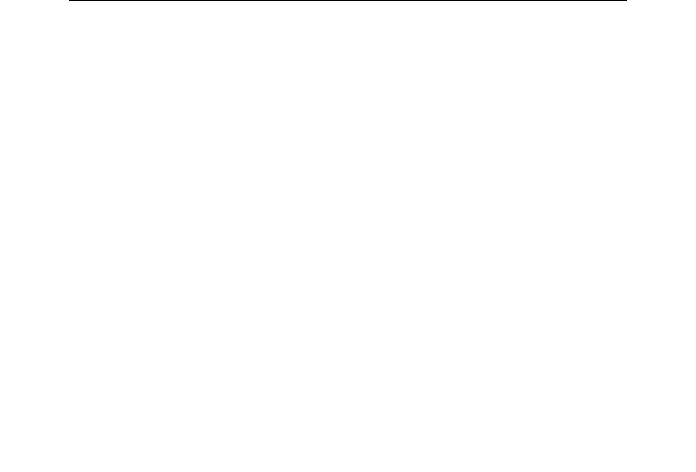
\includegraphics[width= 0.33\textwidth]{Plots/MCReweight/GenInfo/BPpthat.png}
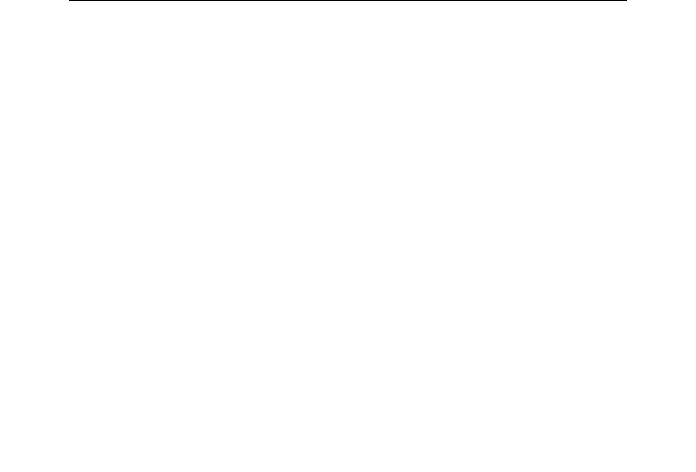
\includegraphics[width= 0.33\textwidth]{Plots/MCReweight/GenInfo/BPJPsiPt.png}
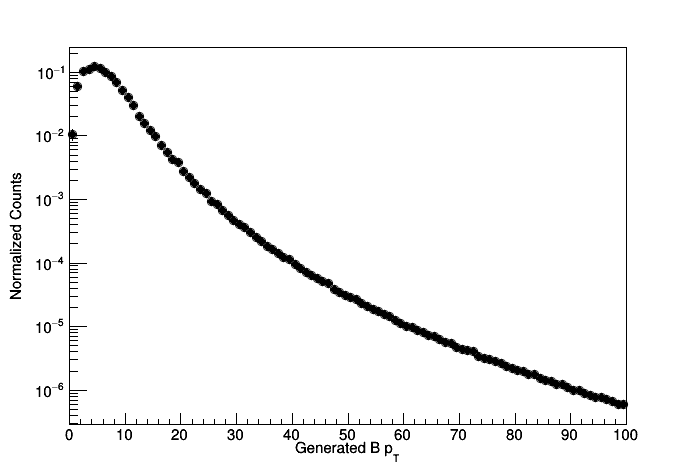
\includegraphics[width= 0.33\textwidth]{Plots/MCReweight/GenInfo/BPGpt.png}
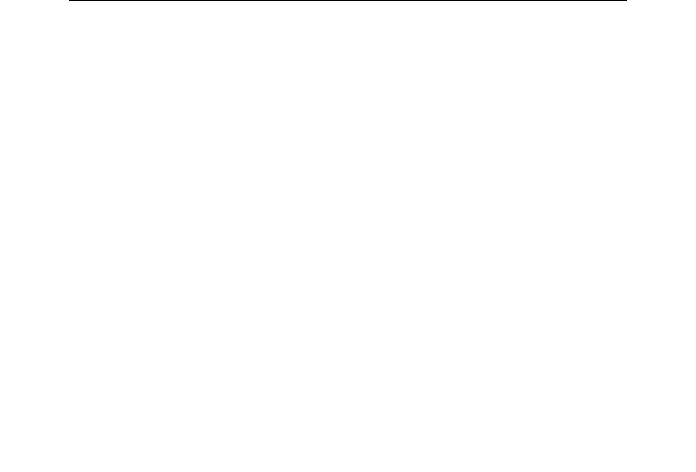
\includegraphics[width= 0.33\textwidth]{Plots/MCReweight/GenInfo/Bspthat.png}
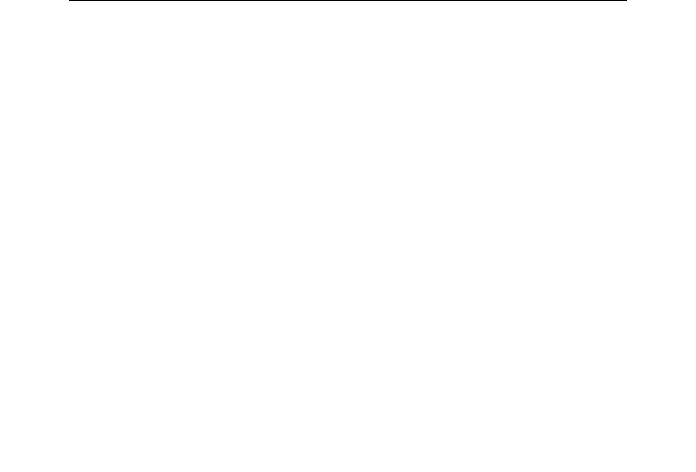
\includegraphics[width= 0.33\textwidth]{Plots/MCReweight/GenInfo/BsJPsiPt.png}
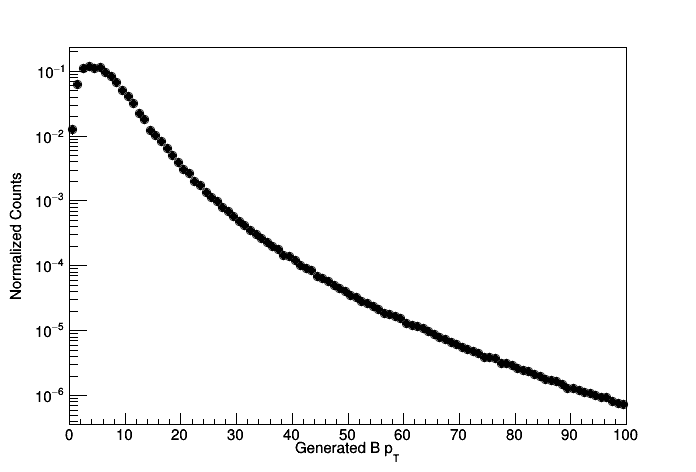
\includegraphics[width= 0.33\textwidth]{Plots/MCReweight/GenInfo/BsGpt.png}
\caption{The pthat distribution of the official MC sample (left) as well as the generated $J/\psi$ (middle) and B-meson \pt distribution with pthat weight applied of $B^{+}$ and $B^0_s$ are shown respectfully above.}
\label{fig:pthatWeightPlot}
\end{center}
\end{figure}

We can see that after $\hat \pt$ reweighting, the Gen \pt distributions have become smoother. This validate our $\hat \pt$ reweighting procedures. 


%Then, we take the ratio of the normalized data raw yield to the normalized MC raw yield and perform a variety of functions to fit the distribution. In our studies, we use Linear ($y = p_0 + p_1 x$), Quadratic ($y = p_0 + p_1 x + p_2 x^2$), Linear + Inverse  ($y = p_1 x + \frac{p_2}{x}$), Linear + Square Root ($y = p_0 + p_1 x + p_2 \sqrt{x}$), Linear + Log ($y = p_0 + p_1 x + p_2 \log{x}$). The data vs MC raw yield shape and our fitting results on spectra ratio are show as follows on Fig~ \ref{fig:BptReweightShape}

Then, we take the ratio of the normalized data raw yield to the normalized MC raw yield and perform a fit with function: $y = p_0/x^2 + p_1 log(x) + p_2$. Our fitting results on spectra ratio are show as follows on Fig~ \ref{fig:BptReweightShape}


\begin{figure}[h]
\begin{center}
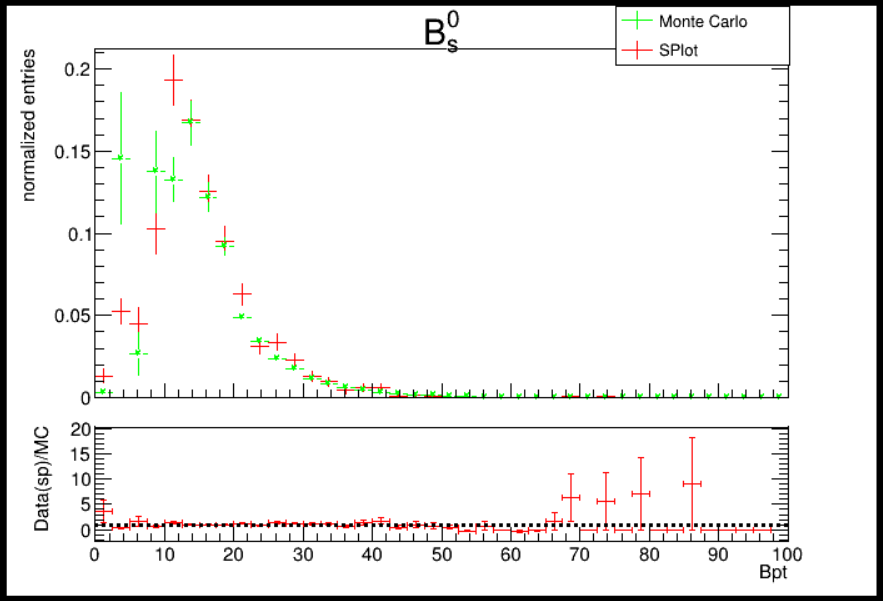
\includegraphics[width= 0.45\textwidth]{Plots/MCReweight/Bpt/BPPtDataMC.png}
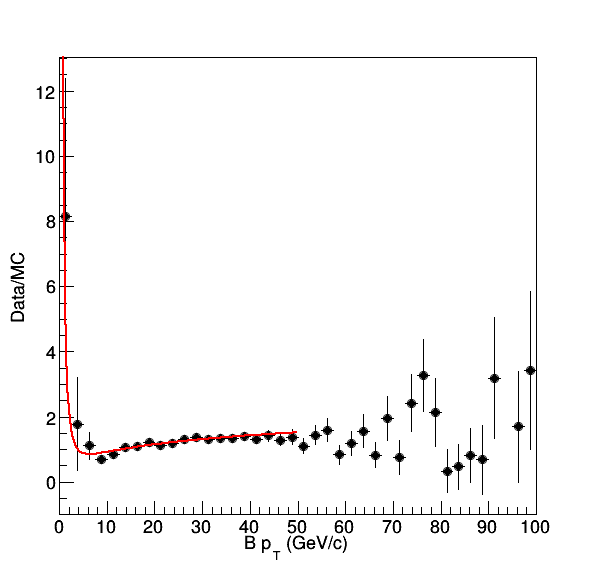
\includegraphics[width= 0.45\textwidth]{Plots/MCReweight/Bpt/BPPtWeight.png}
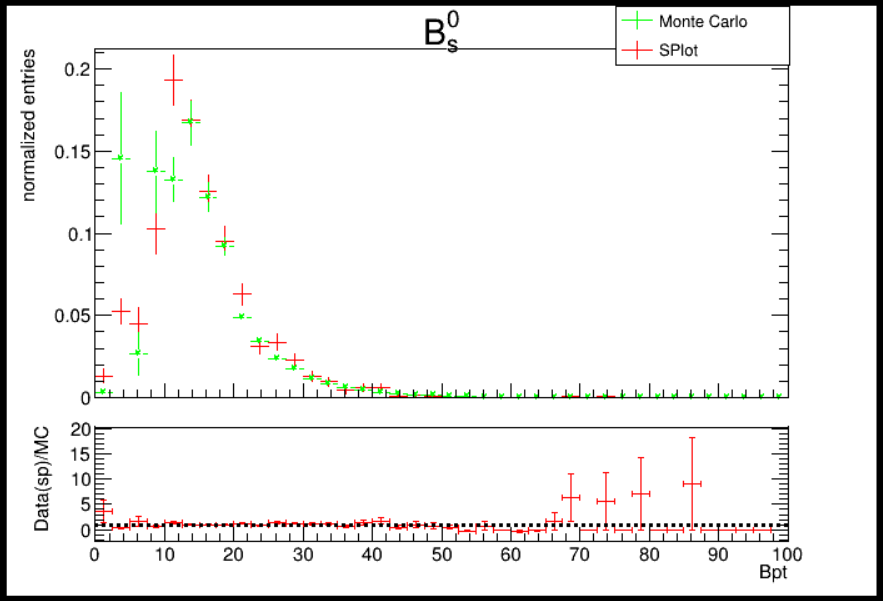
\includegraphics[width= 0.45\textwidth]{Plots/MCReweight/Bpt/BPPtDataMC.png}
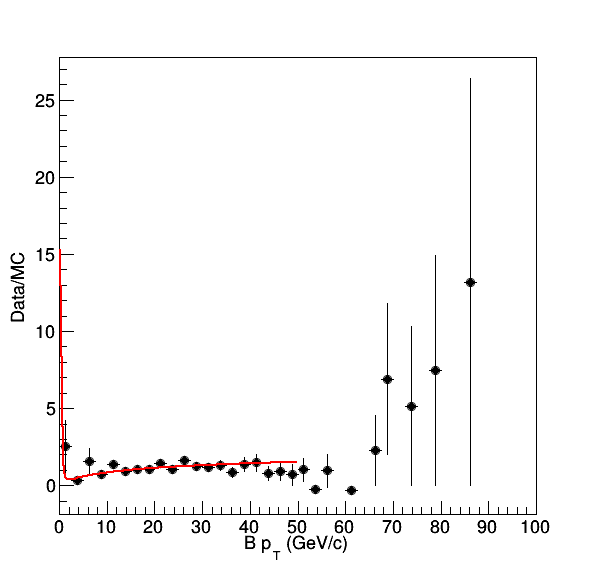
\includegraphics[width= 0.45\textwidth]{Plots/MCReweight/Bpt/BsPtWeight.png}
\caption{The MC-Data agreement between the signal raw yield in data (red) and MC (green) as a function of B meson $p_{T}$ for $B^{+}$ (up) and $B^0_s$ (down). We fit the ratio with the function: $y = p_0/x^2 + p_1 log(x) + p_2$. We will apply this function to the efficiency correct to obtain the systematic uncertainties due to the B $p_T$ shapes.}
\label{fig:BptReweightShape}
\end{center}
\end{figure}


The fitting parameters for all functions are shown below on Table~ \ref{fig:BptReweighTable}



\begin{table}[h]
\begin{center}
\caption{Summary of fitting parameters for the fitting functions of $B^+$ and $B^0_s$ above is shown below.}
\vspace{1em}
\label{fig:BptReweighTable}
\begin{tabular}{| c | c | c | c| }
\hline
Particles & $p_0$ & $p_1$ & $p_2$  \\
\hline
$B^{+}$ &  8.65  &  4.26 & -1.48  \\
$B^0_s$  &  1.00 & 0.436 & 0.171    \\
\hline
\end{tabular}
\end{center}
\end{table}

\clearpage




In addition to above pt shape and centrality reweighting, there must be a primary vertex z position (PVz) reweighting.
It is known there will be some non-trivial disagreement on the primary vertex between data and MC simulated with PYTHIA 8. Also, the offsets between data and MC in the X and Y directions are observed in the 2017 pp collisions. A Gaussian fit is applied to both the data and MC PVz distributions, as showed in Fig.~\ref{fig:datamc-pvz-pp}. The blue markers represent the distribution points for data (left) and MC (middle), while the red lines represents the Gaussian fit results. \note{Add table with fit results} Then, the ratio between the two fit results is taken as the weighting function. Finally, we use the ratio function of reweigh the MC and plot the reweighted MC along with the data on the right window. 
The result after this weighting can be found in Fig. \ref{fig:datamc-pvz-pp} for $B^+$ (up) and $B^0_s$ (down). The Gaussian fit results are given by:

\begin{table}[h]
\begin{center}
	\caption{Summary of fitting parameters for the Gaussian functions ($y = N e^{\frac{-(x-\mu)^2}}{2 \sigma^2}$) of $B^+$ and $B^0_s$ }
\vspace{1em}
\label{fig:BptReweighTable}
\begin{tabular}{| c | c | c | c| }
\hline
	Gaussian Fitting Parameters & N & $\mu$ & $\sigma$ \\
\hline
$B^+$ Data & 0.0132  &  0.7538 & 6.024 \\
$B^+$ MC &  0.0137 & 0.6197 & 5.813 \\
$B^0_s$ Data &  0.0132 & 0.7539 & 6.024  \\
$B^0_s$ MC &  0.0137 & 0.6205 & 5.815    \\
\hline
\end{tabular}
\end{center}
\end{table}



%On the right is the ratio between MC and data, a good agreement is observed.

But note that this analysis is not sensitive to the absolute value of the PV position because the reconstruction of the \Bs meson rely only on the relative distance between PV and \Bs reconstructed vertex which is presented in the following section.
%\textcolor{red}{We tried to estimate this effect by removing this re-weighting entirely and found that the difference is only 1.3\%.}\comment{Do we need to calculate this?}

\begin{figure}[h]
\begin{center}
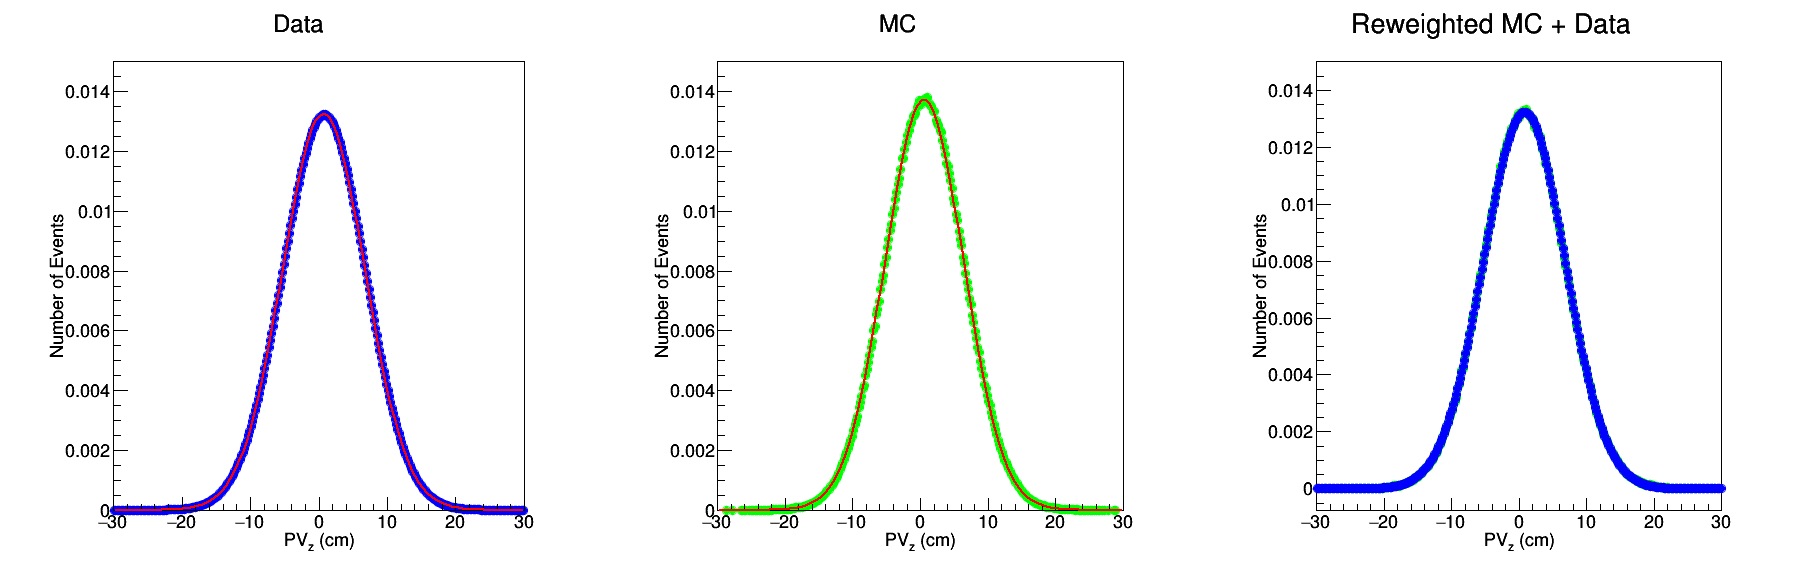
\includegraphics[width= 0.97\textwidth]{Plots/MCReweight/PVz/BPPVZMCData.png}
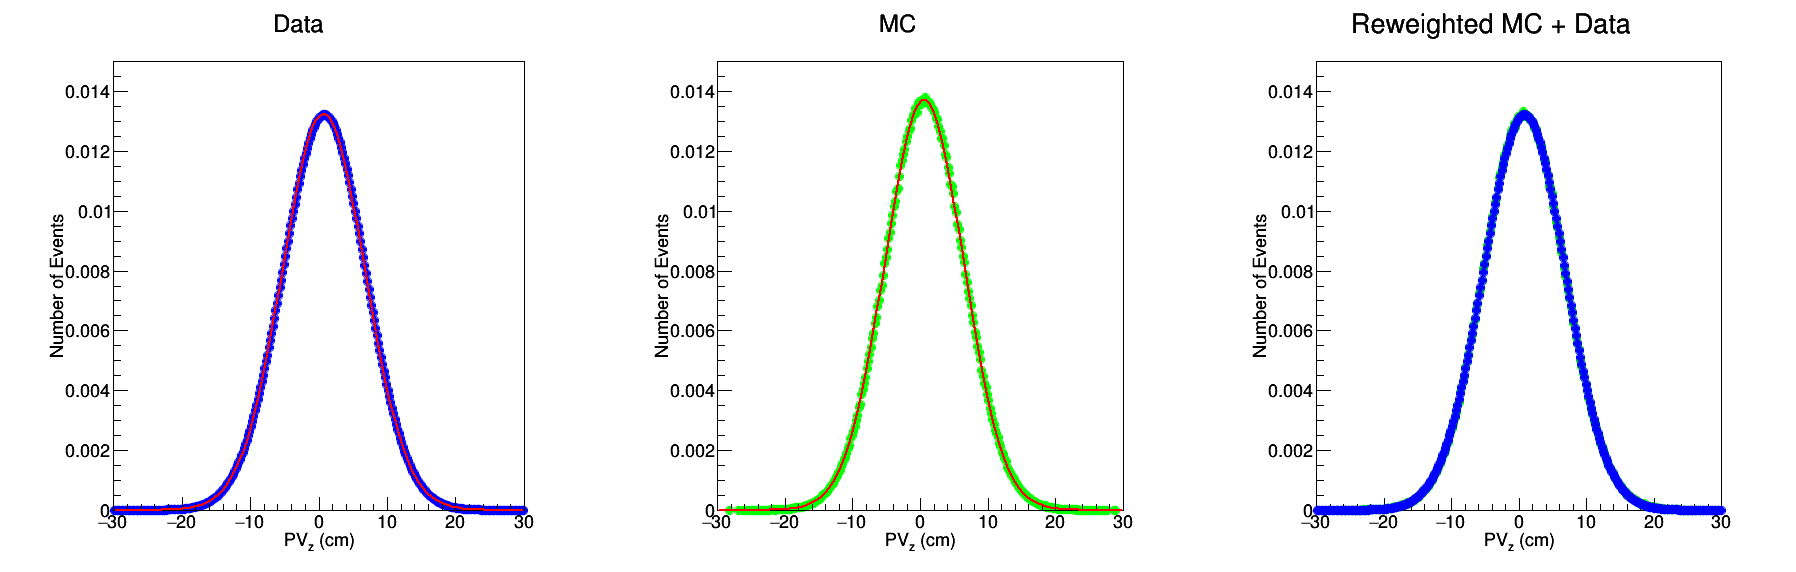
\includegraphics[width= 0.97\textwidth]{Plots/MCReweight/PVz/BsPVZMCData.png}
\caption{ 
On the left, \PBzs primary vertex z position (PVz) spectrum obtained in pp data (geen marker), fitted with a gaussian function (red line). On the middle, the same but for the MC simulations. One the right is the MC and data after reweighting the MC to data with ratio of data-to-MC Gaussian Fits. 
}
\label{fig:datamc-pvz-pp}
\end{center}
\end{figure}

\clearpage

In this case, we can see that there is no need to reweight PVz due to the excellent data MC agreement.
\clearpage


\section{\Bplus meson reconstruction}

In this section, the \Bplus and \PBzs mesons reconstruction strategy are presented. 
The schematic diagram of the workflow is shown in Fig.~\ref{fig:workflow}, starting from muons and tracks to \Bplus meson candidates. 
Muon candidates and tracks are required to pass several quality selection criteria as described in Section~\ref{sec:muonsel} and Section~\ref{sec:tracksel}. 
\Jpsi candidates are reconstructed by vertexing muon pairs with opposite charge, using {\footnotesize KinematicConstrainedVertexFitter}.
The \Bplus candidates are built by combining the \Jpsi candidates with each of the selected tracks.
Finally, a kinematic fit to the \Jpsi-$K^+$ system is performed, forcing the mass of dimuon pair to be equal to to the nominal \Jpsi mass based on PDG~\cite{PDG:2018}.
The selection criteria of the \Bplus candidates are described in Section~\ref{sec:Bsel}. \\

\begin{figure}[h]
\centering
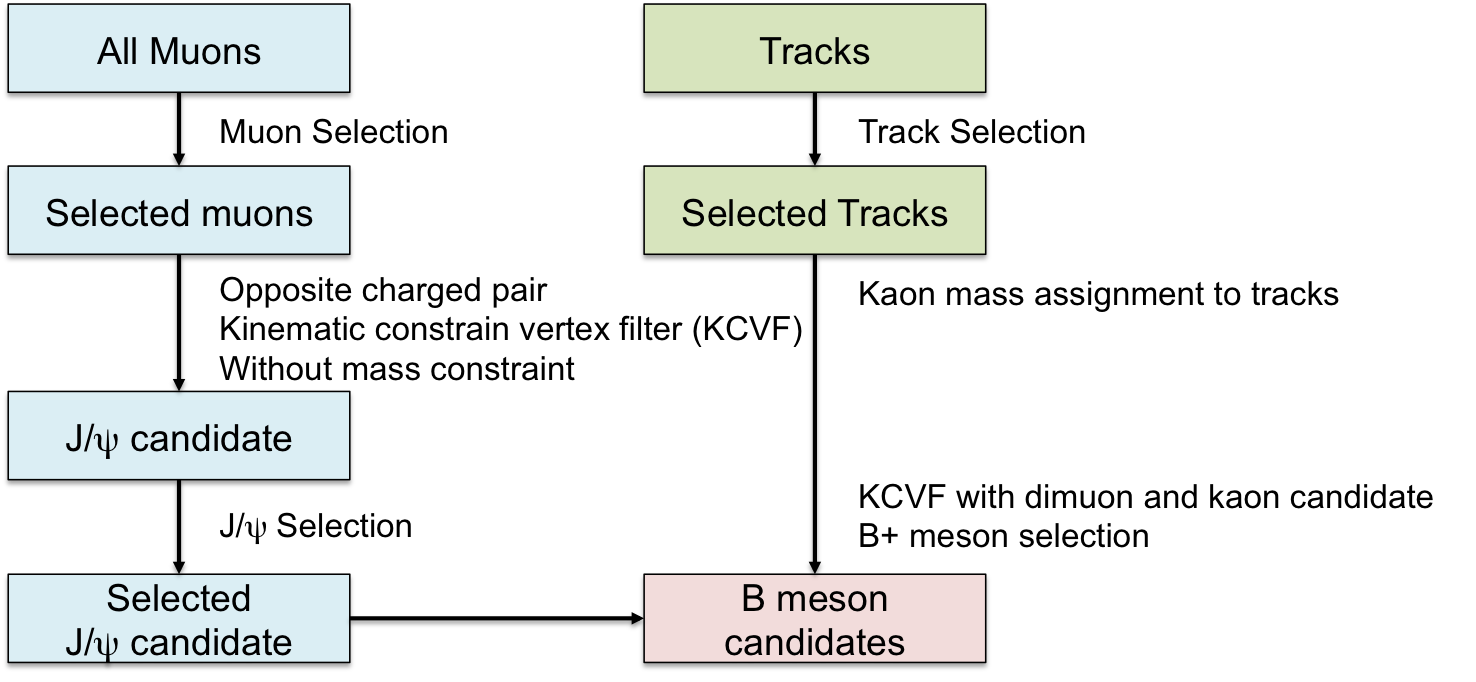
\includegraphics[width=0.9\textwidth]{Plots/BmesonReconstruction/BP.png}
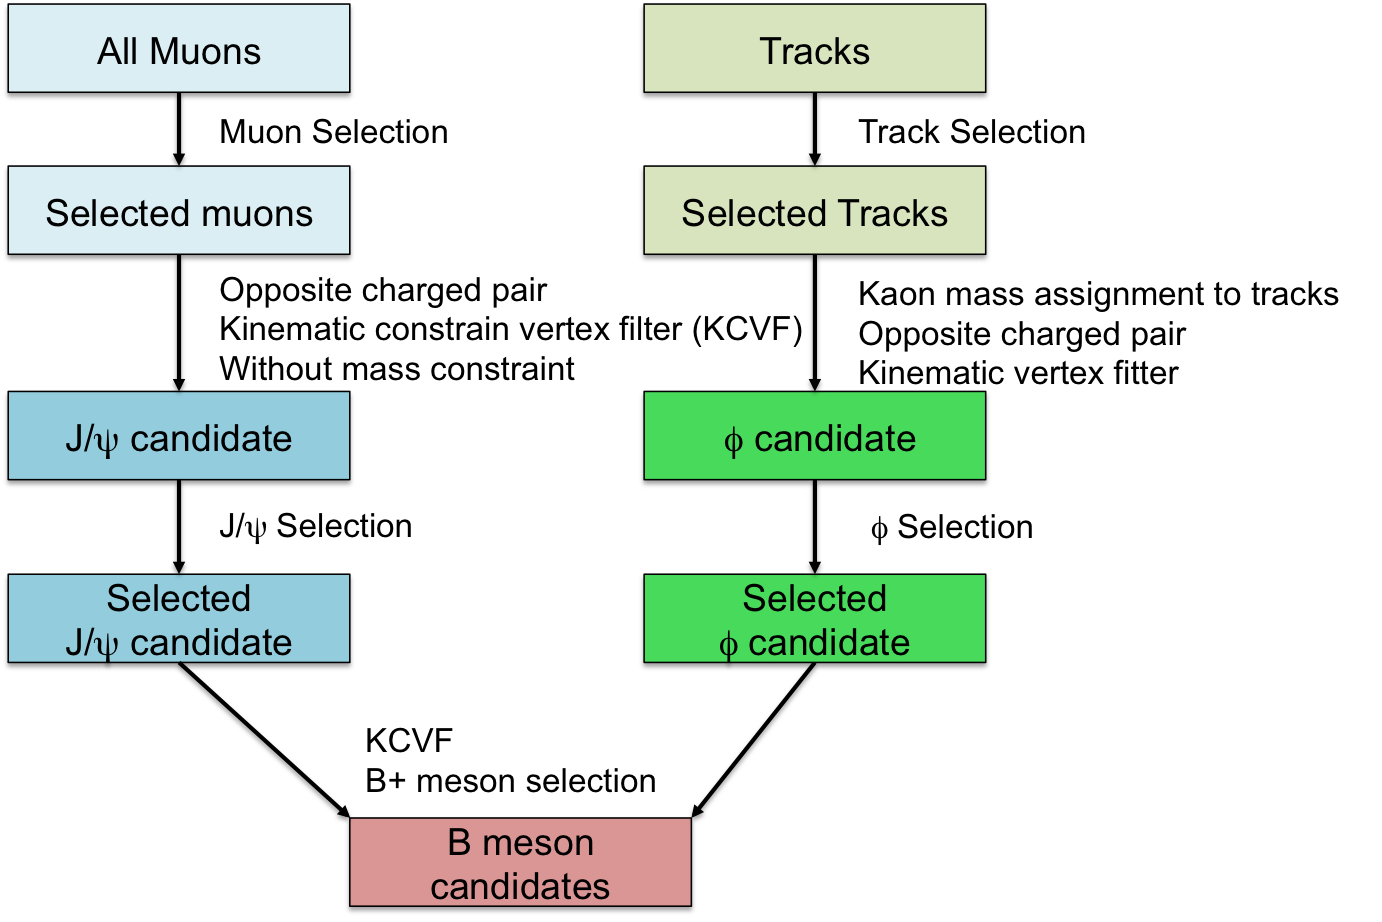
\includegraphics[width=0.9\textwidth]{Plots/BmesonReconstruction/Bs.png}
\caption{Schematic diagrams of the $B^+$ meson (top) and $B^0_s$ reconstruction workflows}
\label{fig:workflow}
\end{figure}


\subsection{Muon and \Jpsi selection}
\label{sec:muonsel}

The muon candidates are selected according to the {\it{hybrid-soft muon selection}}, developed for the muon analyses on the 2017 5.02\TeV data analyses~\cite{AN-16-048}. It is adapted from the soft-muon ID developed in the BPH group, with two modifications: a) the purity selection is removed, and b) the muon is required to be also global. 
The {\it{hybrid-soft muon selection}} includes the following cuts:
\begin{itemize}
\item \textit{isGlobalMuon} and \textit{isTrackerMuon};
\item \textit{isGoodMuon} $> 0$;
\item transverse impact parameter \textit{$\rm D_{xy}$} $< 0.3$;
\item longitudinal impact parameter \textit{$\rm D_{z}$} $< 20$;
\item \textit{nPixWMea} $> 0$ and \textit{nTrkWMea} $> 5$ (\textit{nPixWMea} and \textit{nTrkWMea} are  the number of pixel layers and strips, with valid hits, crossed by a single muon track)
\end{itemize}

Muons are also requested to fulfill the following acceptance selections:
\begin{equation}
\centering
\setlength\arraycolsep{20pt}
\begin{array}{l c r r}
\pt^{\PGm}>3.5\GeVc & & \text{for}\enspace \abs{\eta^{\PGm}}<1.2 & \\
\pt^{\PGm}>(5.77 - 1.89\times\abs{\eta^{\mu}})\GeVc & &  \text{for}\enspace 1.2\le\abs{\eta^{\PGm}}<2.1 &\\
\pt^{\PGm}>1.8\GeVc & & \text{for}\enspace 2.1\le\abs{\eta^{\PGm}}<2.4 &
\end{array}
\label{eq:SingleMuonAccCuts}
\end{equation}

Muons are required to match specific trigger of the following:
\begin{itemize}
\item \textit{Path: HLT$\_$HLT\_HIL1DoubleMu0\_v1}; \\
\item \textit{Last filter: hltL3f0L3Mu0L2Mu0DR3p5FilteredNHitQ10M1to5 $> 0$}.
\end{itemize}

This single muon selection is chosen in order to guarantee a reasonable (above $\approx10\%$) reconstruction and trigger efficiency for all the selected muons. %~\cite{AN-16-048}.

In addition to single muon quality selections, for a pair of muon candidates, the following selections are performed:
\begin{itemize}
\item the two muons have to have opposite sign;
\item dimuon invariant mass has to be within 0.15 GeV from the PDG \Jpsi mass;
\item probability of the two muon tracks to originate from the same decay vertex $>$ 1\%.
\end{itemize}


\subsection {Track selection}
\label{sec:tracksel}
%The track selection we applied are the same with $B^0_{s}$ AN~\cite{AN-19-055}.



Tracks were selected according to the following criteria, as recommended by the HIN tracking group:
\begin{itemize}
\item transverse momentum trkPt $> 0.2$, pseudorapidity $|\eta|$ $< 2.4$;
\item relative uncertainty on the track \pt, (trkPtError/trkPt) $< 0.1$;
\item sum of the numbers of Pixel and Strip hit $> 10$;
\item $\chi^2$ probability normalized by number of degrees of freedom and sum of the numbers of Pixel and Strip Layer hit $> 0.18$.
\end{itemize}

\subsection {$J/\psi$ and $\phi$ selection}

Finally, we also apply selections on the dimuon and dikaon tracks (for $B^0_s$ only):

\begin{itemize}
\item $|m_{\mu\mu} - m_{J/\psi}| < 0.15 GeV/c^{2}$
\item $|m_{K^{+}K^{-}} - m_{\phi}| < 0.015 GeV/c^{2}$
\end{itemize}




\clearpage

\section {\Bplus meson selection}
\label{sec:Bsel}
The selections described in the previous section (so-called prefilter) are not sufficient to distinguish signal from background, especially at low \pt range where the entire spectrum is dominated by combinatorial backgrounds which arises from random combination of muons and tracks. In order to see clear signals and reduce the uncertainties, several additional selection on the \Bplus decay topology were then applied.
A cut optimization procedure was performed to decide the cut values. For more details, see Section ~\ref{sec:CutOpt}.

\subsection{Cut optimization}
\label{sec:CutOpt}
The goal of the optimization procedure is to maximize the figure of merit $S/\sqrt{S+B}$ of the signals while keeping reasonably high signal efficiencies. The optimal cut that minimizes background efficiency for a specific signal efficiency is obtained by the TMVA(Toolkit for Multivariate Data Analysis with ROOT)~\cite{Hocker:2007ht}. \\
Boosted Decision Tree(BDT) is chosen to be the classification method in TMVA training for \Bplus. The reconstructed candidates matched to the generated signal in MC sample are used as signal when training, while the reconstructed candidates in sideband (0.15 GeV/c$^2$ $<$ $|M_{B^{+}}-M_{B^{+}}^{PDG}|$ $<$ 0.25 GeV/c$^2$) of data sample are used as background.

The kinematic variable distributions of daughter tracks and $B^+$ mesons before and after applying the prefilter is shown on Figure~\ref{fig:KinematicsDisMuon1},~\ref{fig:KinematicsDisMuon2},~\ref{fig:KinematicsDisKaon}, ~\ref{fig:KinematicsDisBP}

\clearpage


\begin{figure}[h]
\begin{center}
\includegraphics[width=0.45\textwidth]{Plots/CutOpt/PreFilteredPlots/Bmu1pt_0.png}
\includegraphics[width=0.45\textwidth]{Plots/CutOpt/PreFilteredPlots/Bmu1pt_1.png}
\includegraphics[width=0.45\textwidth]{Plots/CutOpt/PreFilteredPlots/Bmu1eta_0.png}
\includegraphics[width=0.45\textwidth]{Plots/CutOpt/PreFilteredPlots/Bmu1eta_1.png}
%\includegraphics[width=0.45\textwidth]{Plots/CutOpt/PreFilteredPlots/Bmu1phi_0.png}
%\includegraphics[width=0.45\textwidth]{Plots/CutOpt/PreFilteredPlots/Bmu1phi_1.png}
\caption{The normalized $J/\psi$ $\mu^-$ kinematic variable distributions before and after prefilter for \pt = 7 - 10 GeV/c (left) and 10 - 50 GeV/c (right) are shown above.}
\label{fig:KinematicsDisMuon1}
\end{center}
\end{figure}


\clearpage

\begin{figure}[h]
\begin{center}
\includegraphics[width=0.45\textwidth]{Plots/CutOpt/PreFilteredPlots/Bmu2pt_0.png}
\includegraphics[width=0.45\textwidth]{Plots/CutOpt/PreFilteredPlots/Bmu2pt_1.png}
\includegraphics[width=0.45\textwidth]{Plots/CutOpt/PreFilteredPlots/Bmu2eta_0.png}
\includegraphics[width=0.45\textwidth]{Plots/CutOpt/PreFilteredPlots/Bmu2eta_1.png}
%\includegraphics[width=0.45\textwidth]{Plots/CutOpt/PreFilteredPlots/Bmu2phi_0.png}
%\includegraphics[width=0.45\textwidth]{Plots/CutOpt/PreFilteredPlots/Bmu2phi_1.png}
\caption{The normalized $J/\psi$ $\mu^+$ kinematic variable distributions before and after prefilter for \pt = 7 - 10 GeV/c (left) and 10 - 50 GeV/c (right) are shown above.}
\label{fig:KinematicsDisMuon2}
\end{center}
\end{figure}



\clearpage

\begin{figure}[h]
\begin{center}
\includegraphics[width=0.45\textwidth]{Plots/CutOpt/PreFilteredPlots/Btrk1Pt_0.png}
\includegraphics[width=0.45\textwidth]{Plots/CutOpt/PreFilteredPlots/Btrk1Pt_1.png}
\includegraphics[width=0.45\textwidth]{Plots/CutOpt/PreFilteredPlots/Btrk1Eta_0.png}
\includegraphics[width=0.45\textwidth]{Plots/CutOpt/PreFilteredPlots/Btrk1Eta_1.png}
%\includegraphics[width=0.45\textwidth]{Plots/CutOpt/PreFilteredPlots/Btrk1Phi_0.png}
%\includegraphics[width=0.45\textwidth]{Plots/CutOpt/PreFilteredPlots/Btrk1Phi_1.png}
\caption{The normalized $K^+$ track, muons, and $K^+$ track kinematic variable distributions before and after prefilter for \pt = 7 - 10 GeV/c (left) and 10 - 50 GeV/c (right) are shown above.}
\label{fig:KinematicsDisKaon}
\end{center}
\end{figure}

\clearpage

\begin{figure}[h]
\begin{center}
\includegraphics[width=0.45\textwidth]{Plots/CutOpt/PreFilteredPlots/Bpt_0.png}
\includegraphics[width=0.45\textwidth]{Plots/CutOpt/PreFilteredPlots/Bpt_1.png}
\includegraphics[width=0.45\textwidth]{Plots/CutOpt/PreFilteredPlots/By_0.png}
\includegraphics[width=0.45\textwidth]{Plots/CutOpt/PreFilteredPlots/By_1.png}
%\includegraphics[width=0.45\textwidth]{Plots/CutOpt/PreFilteredPlots/Bphi_0.png}
%\includegraphics[width=0.45\textwidth]{Plots/CutOpt/PreFilteredPlots/Bphi_1.png}
\caption{The normalized  $B^+$ kinematic variable distributions before and after prefilter for \pt = 7 - 10 GeV/c (left) and 10 - 50 GeV/c (right) are shown above.}
\label{fig:KinematicsDisBP}
\end{center}
\end{figure}
\clearpage

We can see that the prefilter cuts do not significantly change the distribution of the kinematic variable shapes and create potential bias. Therefore, these show that our prefilter cut is valid to use. 

Then, we use the following six selection variables trained for PbPb:
\begin{itemize}
\item dls3D: Normalized decay length (SV PV distance), the distance between primary and $B^{+}$ decay (secondary) vertex normalized by its uncertainty
\item Balpha: The angle between $B^{+}$ meson displacement and $B^{+}$ meson momentum in 3D
\item Btrk1Pt: Track $p_{T}$, the transverse momentum of the track
\item Bchi2cl: $\chi2$ probability, the $\chi2$ probability of the secondary decay vertex fitting
\item Btrk1Eta: The absolute value of the track pseudorapidity
\item Btrk1Dxysig: Normalized track Dxy, the transverse distance between track and the primary vertex normalized by its uncertainty
\end{itemize}

Same thing for $B^0_s$. HG

The BDT training setup for all \pt bins are as follows: NTree = 850, MinNodeSize=2.5\%, MaxDepth=3, BoostType=AdaBoost, AdaBoostBeta=0.5, UseBaggedBoost, BaggedSampleFraction=0.5, SeparationType=GiniIndex, nCuts=20

The optimal BDT cut values are defined as the numbers which maximize the figure of merit(statistical significance) $S/\sqrt{S+B}$. Here, $S$ is the number of signal in signal region after applying optimal cuts, while $B$ is the number of background in signal region after applying optimal cuts. Signal region is defined as $|M_{B^{+}}-M_{B^{+}}^{PDG}|$ $<$ 0.08 GeV/c$^2$. For the lowest \pt bin, we used a new figure of merit $S/\sqrt{\gamma_{quantile}(\alpha/2,S+B,1)}$ (where, $\alpha$ is chosen to be 1-0.6827) that is suitable for this low signal/background ratio. 

\begin{itemize}
\item $S$ = $S'$ $\times$ (signal optimal cut efficiency), where $S'$ is the number of signal in signal region before applying optimal cuts.
\item $B$ = $B'$ $\times$ (background optimal cut efficiency), where $B'$ is the number of background in signal region before applying optimal cuts.
\end{itemize}

$S'$ and $B'$ are calculated by fitting the invariant mass plot with prefilter selection, with the same functional form used in the main analysis. However, at the 4 lowest \pt bins, the prefilter is not sufficient to reveal the signal. In those cases, $S'$ is calculated by the expected number of signal from FONLL pp cross-section calculation multiplied by pre-filters efficiency, acceptance from MC, and expected \raa value from previous measurement ~\cite{CMS-PAS-HIN-16-011}. \\
Fig.~\ref{fig:tmvaPbPbCorr1} and Fig.~\ref{fig:tmvaPbPbCorr8} show the correlation matrices of the training, in the lowest and highest \pt bin, respectively.

\begin{figure}[h]
\begin{center}
\includegraphics[width=0.45\textwidth]{Plots/CutOpt/CorrelationMatrixB1.pdf}
\includegraphics[width=0.45\textwidth]{Plots/CutOpt/CorrelationMatrixS1.pdf}
\caption{TMVA training correlation matrices of PbPb in \pt 5 - 7 GeV/c.}
\label{fig:tmvaPbPbCorr1}
\end{center}
\end{figure}

\begin{figure}[h]
\begin{center}
\includegraphics[width=0.45\textwidth]{Plots/CutOpt/CorrelationMatrixB8.pdf}
\includegraphics[width=0.45\textwidth]{Plots/CutOpt/CorrelationMatrixS8.pdf}
\caption{TMVA training correlation matrices of PbPb in \pt 20 - 50 GeV/c.}
\label{fig:tmvaPbPbCorr8}
\end{center}
\end{figure}

\clearpage
Fig.~\ref{fig:tmvaPbPbOvertrain18} shows the overtraining check in the lowest and the highest \pt bin. \\

\begin{figure}[h]
\begin{center}
\includegraphics[width=0.45\textwidth]{Plots/CutOpt/overtrain_BDT1.pdf}
\includegraphics[width=0.45\textwidth]{Plots/CutOpt/overtrain_BDT8.pdf}
\caption{TMVA overtraining check of PbPb in \pt 5-7 and 50 - 100 GeV/c, respectively}
\label{fig:tmvaPbPbOvertrain18}
\end{center}
\end{figure}

Fig.~\ref{fig:tmvaPbPbvar4} shows the variable distribution comparison between signal and background, and the statistical significance curve in \pt 15-20GeV. Some variables show prominetly distinct distribution between signal and background. \\

\begin{figure}[h]
\begin{center}
\includegraphics[width=0.90\textwidth]{Plots/CutOpt/variables_id_c1_4.pdf}
\caption{TMVA training variable distribution of PbPb in \pt 15 - 20 GeV/c.}
\label{fig:tmvaPbPbvar4}
\end{center}
\end{figure}

\clearpage
The maximum significance point is selected as our nominal working point, as shown in Fig.~\ref{fig:tmvaPbPbsig4}. \\
Tab.~\ref{tab:cutoptPbPb} shows the summary of the optimal selection criteria in different $p_{T}$ intervals. \\
All the other TMVA performance plots not listed in this section are on Appendix.~\ref{sec:tmvaresults}. \\

\begin{figure}[h]
\begin{center}
\includegraphics[width=0.45\textwidth]{Plots/CutOpt/mvaeffs_BDT4.pdf}
\caption{TMVA significance curve of PbPb in \pt 15 - 20 GeV/c.}
\label{fig:tmvaPbPbsig4}
\end{center}
\end{figure}

\begin{table}[h]
\centering
\begin{tabular}{|c|c|c|c|c|c|c|c|c|}
\hline
\textbf{$p_{T}$ (GeV/c)} & \textbf{5-7} & \textbf{7-10} & \textbf{10-15} & \textbf{15-20} & \textbf{20-30} & \textbf{30-40} & \textbf{40-50} & \textbf{50-60} \\
\hline
BDT & $>$0.02 & $>$0.03 & $>$0.09 & $>$0.07 & $>$0.10 & $>$0.16 & $>$0.20 & $>$0.27 \\
\hline
\end{tabular}
\caption{Summary table of selection criteria in different $p_{T}$ intervals in PbPb collisions}
\label{tab:cutoptPbPb}
\end{table}

\clearpage

\subsection{Fiducial region}
As we go to low \Bplus \pt where the daughter particles also have predominantly low \pt, it becomes improbable to detect muons in low rapidity ranges due to the limited acceptance of the muons. In other words, the signal and background candidates of \Bplus are largely confined to forward rapidity region at low \Bplus \pt. Fig~\ref{fig:2DBeforeCut} shows theoretically possible inverse of acceptance, selection efficiency, and total efficiency vs $B^{+}$ \pt and $|y|$ 2D distribution with only single muon and track selections but without BDT selections. 

\begin{figure}[h]
\begin{center}
\includegraphics[width=0.33\textwidth]{Plots/2DBeforeCut/Acc_0_90.pdf}
\includegraphics[width=0.33\textwidth]{Plots/2DBeforeCut/Sel_0_90.pdf}
\includegraphics[width=0.33\textwidth]{Plots/2DBeforeCut/Eff_0_90.pdf}
\caption{The two dimensional maps of the inverse of the acceptance efficiency (left), selection efficiency (middle), and total efficiency (right) vs \Bplus \pt and rapidity in MC for the centrality range of 0 - 90\% without applying BDT cuts are shown above.}
\label{fig:2DBeforeCut}
\end{center}
\end{figure}


Next, we quantitatively examine the 2D maps of candidate distributions in both data and MC after applying the optimal BDT selections, which are shown in Fig.~\ref{fig:2Dmap}. \\
It is found that \Bplus acceptance is better than \Bs, presumably because of less number of tracks needed to reconstruct B meson, which allows broader phase space that the daughter particles can reside. Since this analysis is mainly for the comparison with \Bs, we adopted more strict fiducial region ($5<$ $p_{T}$ $<10$GeV, 1.5$<$ $|y_{lab}|$ $<$2.4) that is defined using \Bs 2D map. \\

\begin{figure}[h]
\begin{center}
\includegraphics[width=0.45\textwidth]{Plots/invEff/hMass2D_Cent0-90.pdf}
\includegraphics[width=0.45\textwidth]{Plots/invEff/hMass2D_mc_hyperfine_Cent0-90.pdf}
\caption{\Bplus \pt and rapidity two dimensional map of candidates that passed the full analysis cut in data (Left) and MC (right).}
\label{fig:2Dmap}
\end{center}
\end{figure}

\clearpage

\section{MC-Data Comparison}
\label{sec:mcdatacomparison}
\subsection{B candidate properties comparison between data and MC}
Potential differences between Data and MC distributions of the variables used for the selection of the $\Bplus$ signal, can introduce biases in the efficiency corrections. In this section, the distributions of the $\Bplus$ selection variables in PbPb data and MC samples are compared. \\

The Splot method is used for our analysis. This is a likelihood-based method by which we reweight the data using the unbinned fit result. The weights are added to the dataset based on model and yield extraction variables. Each event has two weights: probability of belonging to the signal given its mass, probability of belonging to the background given its mass. The Splot class gives us the distributions of our variables for a given species (signal or background). The advantage of using this method is that we use the full dataset for the comparison in contrast to the sideband subtraction method where one should select the investigation range of signal and background. Furthermore, we use likelihood to describe events' behavior in contrast to the potential misidentification of signal events in background region which might occur in sideband subtraction method. For more details on general description of Splot method applied to this analysis, please refer to the section 4 and 5 of the analysis note CMS AN-19-219(~\cite{AN-19-219}). \\

To show the correlations between the BDT variables to the $B^+$ invariant mass and validate our Splot techniques approach, we first make the correlation matrices for BDT variables vs $B^+$ invariant mass Bmass for data and MC as follows in Figure~\ref{fig:CorrMatrice_BDT}:

\begin{figure}[h]
\begin{center}
\includegraphics[width=0.45\textwidth]{Plots/SPlots/CorrelationMatrixB.pdf}
\includegraphics[width=0.45\textwidth]{Plots/SPlots/CorrelationMatrixS.pdf}
\caption{The correlation matrices in data (left) and MC (right) are shown above.}
\label{fig:CorrMatrice_BDT}
\end{center}
\end{figure}

Fig.~\ref{fig:Splot_BDT} shows the data and MC comparison results based on Splot method. Here, we focus on BDT values that are directly used in our signal extraction and related to MC distribution validation, rather than the variables themselves used in BDT training. In a wide ranges of BDT, the two distributions show good agreement. We only focus on the region where BDT is greater than the working point and is smaller than the maximum value that candidates have.

\begin{figure}[h]
\begin{center}
\includegraphics[width=0.45\textwidth]{Plots/SPlots/BDT_pt_5_7_mc_validation_Bu.pdf}
\includegraphics[width=0.45\textwidth]{Plots/SPlots/BDT_pt_7_10_mc_validation_Bu.pdf}
\includegraphics[width=0.45\textwidth]{Plots/SPlots/BDT_pt_10_15_mc_validation_Bu.pdf}
\includegraphics[width=0.45\textwidth]{Plots/SPlots/BDT_pt_15_20_mc_validation_Bu.pdf}
\includegraphics[width=0.45\textwidth]{Plots/SPlots/BDT_pt_20_30_mc_validation_Bu.pdf}
\includegraphics[width=0.45\textwidth]{Plots/SPlots/BDT_pt_30_40_mc_validation_Bu.pdf}
\includegraphics[width=0.45\textwidth]{Plots/SPlots/BDT_pt_40_50_mc_validation_Bu.pdf}
\includegraphics[width=0.45\textwidth]{Plots/SPlots/BDT_pt_50_60_mc_validation_Bu.pdf}
\caption{Comparison of \Bplus BDT distribution in data and MC using Splot method.}
\label{fig:Splot_BDT}
\end{center}
\end{figure}


\iffalse

The sideband subtraction method is a widespread technique used to extract signal distributions from a sample that contains background components. In general, the data sample is split into one or more background regions (so-called, sideband) and one signal region, by using discrimination variables which depends on the analysis undertaken. The method assumes that there is no signal outside the signal region, i.e. all the events which lie in the background regions are background-like. As a consequence, it is reasonable to assume the behavior of the events outside the signal region to be similar to the behaviour of the background events inside the signal region. Under this assumption, by performing an interpolation of the background regions that surround the signal region, one is then able to estimate the amount of background in the signal region. \\
Finally, it is enough to subtract the background estimation from the total data sample in the signal region to obtain the signal distribution. In addition, MC gen-metched B signal candidates (i.e., match to generator level signal $\Bplus$) are also shown in corresponding variables and compared to the data and MC sideband subtracted events. \\
In this analysis, we use the reconstructed mass of the involved \PB meson candidate as the discriminating variable. We have checked the background in the sideband defined as $0.15<$ $|M_{B^+}}-M_{B^+}^{PDG}|$ $<0.25$ (GeV/c$^2$) show desirable behavior (linear), as shown in Fig.~\ref{fig:DataMCComparisonPbPb_sideband}. This justifies the interpolation technique described above. On the other hand, The signal region is chosen to be $|M_{B^+}}-M_{B^+}^{PDG}|$ $<0.08$ (GeV/c$^2$), and their distribution is distinguishable from background in sideband.
In order to extract the signal distributions, the \Bplus yields were extracted as a function of different selection variables using the standard selection criteria in the main results. The distributions were then normalized to unity, to allow a meaningful comparison between data and MC.
Most of the results shown in Fig.~\ref{fig:DataMCComparisonPbPb1}, ~\ref{fig:DataMCComparisonPbPb2}, and ~\ref{fig:DataMCComparisonPbPb3} demonstrate good agreement within uncertainties over a wide range of \pt and a variety of variable.

\begin{figure}[h]
\begin{center}
\includegraphics[width=0.45\textwidth]{Plots/Results/plotFitsComp/MassPlot.png}
\caption{Sideband subtraction scheme for $\Bplus$ in PbPb.}
\label{fig:DataMCComparisonPbPb_sideband}
\end{center}
\end{figure}

\begin{figure}[h]
\begin{center}
\includegraphics[width=0.32\textwidth]{Plots/Results/plotFitsComp/RatioPlotsPullRatio_PbPb_0.pdf}
\includegraphics[width=0.32\textwidth]{Plots/Results/plotFitsComp/RatioPlotsPullBd0Err_PbPb_0.pdf}
\includegraphics[width=0.32\textwidth]{Plots/Results/plotFitsComp/RatioPlotsPullBsvpvDistance_PbPb_0.pdf}
\includegraphics[width=0.32\textwidth]{Plots/Results/plotFitsComp/RatioPlotsPullBalpha_PbPb_0.pdf}
\includegraphics[width=0.32\textwidth]{Plots/Results/plotFitsComp/RatioPlotsPullBchi2cl_PbPb_0.pdf}
\includegraphics[width=0.32\textwidth]{Plots/Results/plotFitsComp/RatioPlotsPullBmu1Eta_PbPb_0.pdf}
\includegraphics[width=0.32\textwidth]{Plots/Results/plotFitsComp/RatioPlotsPullBmu2Eta_PbPb_0.pdf}
\includegraphics[width=0.32\textwidth]{Plots/Results/plotFitsComp/RatioPlotsPullBmu1Pt_PbPb_0.pdf}
\includegraphics[width=0.32\textwidth]{Plots/Results/plotFitsComp/RatioPlotsPullBmu2Pt_PbPb_0.pdf}
\caption{
Comparison of various \Bplus meson variables between data and MC in PbPb analysis in \pt 5-100 GeV/c (1).}
\label{fig:DataMCComparisonPbPb1}
\end{center}
\end{figure}

\begin{figure}[h]
\begin{center}
\includegraphics[width=0.32\textwidth]{Plots/Results/plotFitsComp/RatioPlotsPullBtrk1Dxy1Sig_PbPb_0.pdf}
\includegraphics[width=0.32\textwidth]{Plots/Results/plotFitsComp/RatioPlotsPullBtrk1DxyError1_PbPb_0.pdf}
\includegraphics[width=0.32\textwidth]{Plots/Results/plotFitsComp/RatioPlotsPullBtrk1Dxy1_PbPb_0.pdf}
\includegraphics[width=0.32\textwidth]{Plots/Results/plotFitsComp/RatioPlotsPullBtrk1Dz1_PbPb_0.pdf}
\includegraphics[width=0.32\textwidth]{Plots/Results/plotFitsComp/RatioPlotsPullBtrk1Dz1Sig_PbPb_0.pdf}
\includegraphics[width=0.32\textwidth]{Plots/Results/plotFitsComp/RatioPlotsPullBtrk1DzSig_PbPb_0.pdf}
\includegraphics[width=0.32\textwidth]{Plots/Results/plotFitsComp/RatioPlotsPullBtrk1Eta_PbPb_0.pdf}
\includegraphics[width=0.32\textwidth]{Plots/Results/plotFitsComp/RatioPlotsPullBtrk1Pt_PbPb_0.pdf}
\includegraphics[width=0.32\textwidth]{Plots/Results/plotFitsComp/RatioPlotsPullPVz_PbPb_0.pdf}
\caption{
Comparison of various \Bplus meson variables between data and MC in PbPb analysis in \pt 5-100 GeV/c (2).}
\label{fig:DataMCComparisonPbPb2}
\end{center}
\end{figure}

\begin{figure}[h]
\begin{center}
\includegraphics[width=0.32\textwidth]{Plots/Results/plotFitsComp/RatioPlotsPullBtrk1DzSig_PbPb_0.pdf}
\includegraphics[width=0.32\textwidth]{Plots/Results/plotFitsComp/RatioPlotsPullBtrk1Eta_PbPb_0.pdf}
\includegraphics[width=0.32\textwidth]{Plots/Results/plotFitsComp/RatioPlotsPullBtrk1Pt_PbPb_0.pdf}
\includegraphics[width=0.32\textwidth]{Plots/Results/plotFitsComp/RatioPlotsPullBtrk1Y_PbPb_0.pdf}
\includegraphics[width=0.32\textwidth]{Plots/Results/plotFitsComp/RatioPlotsPullBvtxX_PbPb_0.pdf}
\includegraphics[width=0.32\textwidth]{Plots/Results/plotFitsComp/RatioPlotsPullBvtxY_PbPb_0.pdf}
\includegraphics[width=0.32\textwidth]{Plots/Results/plotFitsComp/RatioPlotsPullBy_PbPb_0.pdf}
\caption{
Comparison of various \Bplus meson variables between data and MC in PbPb analysis in \pt 5-100 GeV/c. (3)}
\label{fig:DataMCComparisonPbPb3}
\end{center}
\end{figure}

\fi

\clearpage

\section{Signal Extraction}
\label{sec:sigextract}
The method and the fit model for signal and background we applied are mostly the same with $B_{s}$ AN. Please refer to the corresponing section in ~\cite{AN-19-055}. \\
However, there is one major difference between $B_{s}$ and \Bplus yield extraction. From the inclusive \Jpsi sample study, we have found that there is a clear and sizable contribution from non-prompt \Jpsi candidates that are fed down from the \Bplus signal in our region of interest. We model this component with an error function and a Gaussian. The error function component mostly comes from 4-prong B meson decay (e.g. $\Bplus\rightarrow\Jpsi~K^{*}(892)^{+}$) that are partially reconstructed as \Bplusdecay (one track is lost) and can form peaking structures for values of the invariant mass below $\approx$5.20 GeV/c$^2$. The Gaussian contribution mainly comes from $\Bplus\rightarrow\Jpsi~\pi^{+}$ where pion is misidentifieds as kaon. \\
The ratio of the height of error function and the Gaussian is fixed by MC simulation. However, the Gaussian component is shown to be relatively negligible compared to the error function, and even more to the signal double Gaussian of our nominal channel. More details on the non-prompt \Jpsi study can be found in Appendix Sec.~\ref{sec:nonprompt}. \\
Note that we do not discriminate $\PBp$ from $\PBm$ in raw yield extraction process. Therefore, the invariant mass plots shown below contains both $\PBp$ and $\PBm$ signal and backgrounds. This double counting is properly canceled in the corrected yield calculation process later. \\

\iffalse
Raw yields are extracted in each $\pt$-interval via a fit procedure. The fit functions consists of the following components:

\begin{itemize}
\item \textit{A double Gaussian with same mean but different widths to model the signal component}. This was preferred to a single/triple gaussian and a Breit-Wigner function since it showed to better describe the signal shape in MC simulations.
\item \textit{An exponential function to describe the combinatorial background}. This background component is mostly produced by the random combination of a \Jpsi candidate with tracks that are not coming from the same \Bplus decay.
\item \textit{An error function + a Gaussian to model the non-prompt J/$\psi$ background component}. The error function component mostly comes from 4-prong B meson decay (e.g. $\Bplus\rightarrow\Jpsi~K^{*}(892)^{+}$) that are partially reconstructed as \Bplusdecay (one track is lost) and can form peaking structures for values of the invariant mass below $\approx$5.20 GeV/c$^2$. The Gaussian contribution mainly comes from $\Bplus\rightarrow\Jpsi~\pi^{+}$ where pion is misidentifieds as kaon. The ratio of areas of the error function and the Gaussian is fixed by MC simulation. However, the Gaussian component is shown to be relatively negligible compared to the error function, and even more to the signal double Gaussian of our nominal channel. More details on the non-prompt \Jpsi study can be found in Appendix Sec.~\ref{sec:nonprompt}.
\end{itemize}

A likelihood fit is used for this analysis. The results were cross-checked with the ones obtained by $\chi^2$ procedure.
The invariant mass range considered for the fits is from 5 to 6 GeV/c$^2$. 
The fit strategy proceeds as follows:

\begin{itemize}
\item First, a fit is performed, with a double gaussian function to the MC invariant mass distribution of the genuine \Bplus signals.
\item The shape of the non-prompt background component is obtained using the dedicated non-prompt \Jpsi MC samples.
\item The fit is performed to the data with the fixed the shape (widths and relative proportion of the two Gaussians) same with the Gaussians obtained from the MC fit.
\item For systematic uncertainty check, add a free parameter (a), that is commonly multiplied to the widths of the signal Gaussians, serving as a scale factor of the resolution that parametrizes data and MC signal shape difference. However in the nominal fit, this is set to be unity, which means the widths of the data signal are set to be identical to the ones of the MC signal.
\item The parameters of the background PDF, the mean of the signal Gaussians are the free parameters of the fit.
\end{itemize}

Unbinned fit by Roofit package available on ROOT is adopted in our signal extraction. 
\fi

In Fig.~\ref{fig:pbpbmass1} and Fig.~\ref{fig:pbpbmass2}, the invariant mass spectra and their pull distributions obtained in the \pt intervals in the PbPb analyses are presented. %In Table ~\ref{tab:chi2_tab}, the $\chi^2$ values for the fits are provided.

\iffalse
\begin{figure}[h]
\begin{center}
\includegraphics[width= 0.45\textwidth]{Plots/Results/plotFits/data_PbPb_1_Bpt_57_doubly0_ntKp.pdf}
\includegraphics[width= 0.45\textwidth]{Plots/Results/plotFits/data_PbPb_2_Bpt_710_doubly0_ntKp.pdf}
\includegraphics[width= 0.45\textwidth]{Plots/Results/plotFits/data_PbPb_3_Bpt_1015_doubly0_ntKp.pdf}
\includegraphics[width= 0.45\textwidth]{Plots/Results/plotFits/data_PbPb_4_Bpt_1520_doubly0_ntKp.pdf}
\caption{Invariant mass distribution of $\Bplus$ candidates obtained in PbPb collisions in \pt intervals in the transverse momentum range from 5-20 GeV/c and Centrality 0-90$\%$.}
\label{fig:pbpbmass1}
\end{center}
\end{figure}

\begin{figure}[h]
\begin{center}
\includegraphics[width= 0.45\textwidth]{Plots/Results/plotFits/data_PbPb_5_Bpt_2030_doubly0_ntKp.pdf}
\includegraphics[width= 0.45\textwidth]{Plots/Results/plotFits/data_PbPb_6_Bpt_3040_doubly0_ntKp.pdf}
\includegraphics[width= 0.45\textwidth]{Plots/Results/plotFits/data_PbPb_7_Bpt_4050_doubly0_ntKp.pdf}
\includegraphics[width= 0.45\textwidth]{Plots/Results/plotFits/data_PbPb_8_Bpt_5060_doubly0_ntKp.pdf}
\caption{Invariant mass distribution of $\Bplus$ candidates obtained in PbPb collisions in \pt intervals in the transverse momentum range from 20-60 GeV/c and Centrality 0-90$\%$.}
\label{fig:pbpbmass2}
\end{center}
\end{figure}
\fi

\begin{figure}[h]
\begin{center}
\includegraphics[width= 0.45\textwidth]{Plots/Results/plotFitsBsBin/data_PbPb_1_Bpt_710_doubly0_0_90_ntKp.pdf}
\includegraphics[width= 0.45\textwidth]{Plots/Results/plotFitsBsBin/data_PbPb_1_Bpt_1015_doubly0_0_90_ntKp.pdf}
\includegraphics[width= 0.45\textwidth]{Plots/Results/plotFitsBsBin/data_PbPb_1_Bpt_1520_doubly0_0_90_ntKp.pdf}
\includegraphics[width= 0.45\textwidth]{Plots/Results/plotFitsBsBin/data_PbPb_1_Bpt_2050_doubly0_0_90_ntKp.pdf}
\caption{Invariant mass distribution of $\Bplus$ candidates obtained in PbPb collisions in \pt intervals in the transverse momentum range from 7-50 GeV/c and Centrality 0-90$\%$.}
\label{fig:pbpbmass1}
\end{center}
\end{figure}

\begin{figure}[h]
\begin{center}
\includegraphics[width= 0.45\textwidth]{Plots/Results/plotFitsBsBin/data_PbPb_1_Bpt_1050_doubly0_0_30_ntKp.pdf}
\includegraphics[width= 0.45\textwidth]{Plots/Results/plotFitsBsBin/data_PbPb_1_Bpt_1050_doubly0_30_90_ntKp.pdf}
\includegraphics[width= 0.45\textwidth]{Plots/Results/plotFitsBsBin/data_PbPb_1_Bpt_1050_doubly0_0_90_ntKp.pdf}
\caption{Invariant mass distribution of $\Bplus$ candidates obtained in PbPb collisions in centrality intervals 0 - 30\%, 30 - 90\%, and 0 - 90\% in the transverse momentum range from 10 - 50 GeV/c.}
\label{fig:pbpbmass2}
\end{center}
\end{figure}


\iffalse

\begin{table}[h]
\begin{center}
\caption{Summary table of $\chi^2$ normalized by degree of freedom after the fitting for each B \pt bins}
\vspace{1em}
\label{tab:chi2_tab}
  \begin{tabular}{ c | c | c | c | c | c | c | c }
    \hline
    Dataset & (5,7) & (7,10) & (10,15) & (15,20) & (20,30)) & (30,50) & (50,100) \\
    \hline
%    pp & N/A & 1.17 & 2.26 & 1.61 & 1.82 & 0.82 & 0.22 \\
    PbPb & 0.76 & 1.06 & 1.42 & 1.02 & 1.57 & 0.90 & 0.10 \\
    \hline
\end{tabular}
\end{center}
\end{table}

\fi

%For \pt and centrality doubly differential signal extraction plots, please refer to \ref{sec:sigdoublediff}.
%For inclusive \pt signal extraction plots, please refer to \ref{sec:inclusivept}.

We also make the comparison between the symmetric raw yield error and their asymmetric upper and lower yield error using the RooFit framework on the unbinned fit. The table is shown below in Table~\ref{tab:ErrorComp}:


\begin{table}[h]
\begin{center}
\caption{The comparison between RooFit and unbinned fit framework.}
\vspace{1em}
\label{tab:ErrorComp}
  \begin{tabular}{| c | c |c | c| c| }
    \hline
     Centrality &  \pt (GeV/c) & Raw Yield Error & RawYield Error Up & Raw Yield Error Down  \\
    \hline
    \hline
0 - 90\% & 7 - 10 & 10.88  & 11.20  & 10.66   \\ 
0 - 90\% & 10 - 15 & 20.68  & 21.05  & 20.35  \\ 
0 - 90\% & 15 - 20 & 17.86 & 18.21  & 17.56  \\ 
0 - 90\% & 20 - 50 & 19.84  & 20.19  &  19.55 \\ 
0 - 30\% & 10 - 50 &  27.72 &  28.01 &  27.45 \\ 
30 - 90\% & 10 - 50 & 19.53 & 19.92 &  19.20 \\ 
0 - 90\% & 10 - 50  & 33.78  & 34.13  & 33.47 \\ 
    \hline
    \hline
\end{tabular}
\end{center}
\end{table}



\clearpage

\subsection{Closure test of the fitting procedure}
In order to validate the yield extraction procedure, we generate 5000 toy MC for the fit and make the pull distribution. Then we perform the Guassian fits to the pull distribution to obtain the mean and width. The results are show in Fig ~\ref{fig:closurepullpt} and Fig ~\ref{fig:closurepullcent}:

\begin{figure}[h]
\begin{center}
\includegraphics[width= 0.40\textwidth]{Plots/ClosureTest/DataBoostrapFit/pull_signal_full_0_0_90.png}
\includegraphics[width= 0.40\textwidth]{Plots/ClosureTest/DataBoostrapFit/pull_signal_full_1_0_90.png}
\includegraphics[width= 0.40\textwidth]{Plots/ClosureTest/DataBoostrapFit/pull_signal_full_2_0_90.png}
\includegraphics[width= 0.40\textwidth]{Plots/ClosureTest/DataBoostrapFit/pull_signal_full_3_0_90.png}
\caption{The pull distribution and the Gaussian fits for 0 - 90\% at 7 - 10, 10 - 15, 15 - 20, 20 - 50 are shown respectfully above.} 
\label{fig:closurepullpt} 
\end{center}
\end{figure}

\clearpage

\begin{figure}[h]
\begin{center}
\includegraphics[width= 0.45\textwidth]{Plots/ClosureTest/DataBoostrapFit/pull_signal_full_-1_0_90.png}
\includegraphics[width= 0.45\textwidth]{Plots/ClosureTest/DataBoostrapFit/pull_signal_full_-1_0_30.png}
\includegraphics[width= 0.45\textwidth]{Plots/ClosureTest/DataBoostrapFit/pull_signal_full_-1_30_90.png}
\caption{The pull distribution and the Gaussian fits for 0 - 90\% at 7 - 10, 10 - 15, 15 - 20, 20 - 50 are shown respectfully above.} 
\label{fig:closurepullcent} 
\end{center}
\end{figure}



We can see that all \pt and centrality bins have zero mean and unit width from the Gaussian fits to the pull distribution. This validate the closure of our fits to extract the $B^+$ raw yield. 




\clearpage

\section{Acceptance and Efficiency}
\label{sec:AccEff}

\clearpage


\section{Closure Test of the $B^{+}$ Corrected Yield}
\label{sec:closuretest}

\subsection{Raw Yield Closure}

\subsection{Efficiency Closure}

\subsection{Corrected Yield Closure}


\clearpage

\section{Results}
\label{sec:results}

%\subsection{dN/d\texorpdfstring{\pt}{Lg} in pp collisions at 5.02 TeV}

\subsection{\pt differential corrected yield in pp collisions at 5.02 TeV}

The method we applied is the same with $B_{s}$ AN~\cite{AN-19-055}.

\iffalse
The $\rm dN/d\pt$ in pp collisions is defined as:

\begin{equation}
  \left.\frac{1}{T_{AA}} \frac{{\rm d}N^{\rm }}{{\rm d}\pt}\right|_{|y|<2.4} =
  \frac{1}{T_{AA}} \frac{1}{2}\frac{1}{\Delta\pt} \frac{\left. N^{\rm \Bplus}\right|_{|y|<2.4}}{(\alpha\times\epsilon) \cdot{\rm BR} \cdot N_{events} \cdot \epsilon_{trigger}}\,
  \label{eq:ppYield}
\end{equation}

where $\rm T_{AA}$ is the nuclear overlap function (Ref. \verb#https://twiki.cern.ch/twiki/bin/viewauth/CMS/GlauberTables#, ~\cite{AN-15-080}). The centrality ranges used in our analysis are summarized in table~\ref{tab:TAA}. The 30-90$\%$ is not available now, so we used 30-100$\%$ as a substitute. The actual cross section value for this centrality will be lower than what we present.
For the $N_{events}$ which is the number of MinimumBias events correspond to the muon json files, we haven't computed this yet. We expect that this will be provided from other source.
%However, there is a previously computed value for 2015 pp Run of $350\mubinv$ (for more info, check out https://twiki.cern.ch/twiki/pub/CMS/HINUpsilonRaa2016/Jason-MinBiasCounting-2017-02-02.pdf). We scaled this number of MinimumBias events along with the luminosity increase from $350\mubinv$ to $1500\mubinv$. The accurate value will be evaluated in the near future.

\begin{table}
\begin{center}
    \begin{tabular}{|c|c|c|c|}
\hline
Centrality & $<N_{coll}>$ & $<T_{AA}> (mb^{-1})$ & $<N_{part}>$ \\
\hline
0 - 90\% & 424.1$\pm$2.2$\%$ & 6.274$\pm$2.2$\%$ & 126.0$\pm$0.67$\%$ \\
\hline
0 - 30\% & 1042$\pm$2$\%$ & 15.41$\pm$2$\%$ & 269.1$\pm$0.38$\%$ \\
\hline
30 - 90\% & 115.3$\pm$3.2$\%$ & 1.705$\pm$3.2$\%$ & 54.44$\pm$1.1$\%$ \\
\hline
    \end{tabular}
\caption{Summary of the $N_{\rm coll}$, $T_{\rm AA}$ and $N_{\rm part}$ values for the centrality bins used in the analysis. Note that the 30-100$\%$ value is used as a substitute of 30-90$\%$.}
\label{tab:TAA}
\end{center}
\end{table}

\fi

In Fig.~\ref{fig:ppxsecpt}, Number of MinBias events-normalized, TAA-normalized, efficiency-corrected and \pt-width divided yield (let's call this ``normalized corrected yield'') of \Bplus mesons in the centrality 0-90\% and rapidity region $\abs{y_\text{lab}}<2.4$ (Caveat: Note the fiducial region $1.5<\abs{y_\text{lab}}<2.4$ in \Bplus \pt 7 - 10GeV/c) in PbPb collisions at \sqrts=5.02 TeV is presented. The boxes around the data points represent the total systematic uncertainties.

\begin{figure}[h]
\begin{center}
%\includegraphics[width= 0.45\textwidth]{Plots/Results/plotCrossSection/canvasSigmaBplusRatiopp_Bplusbin.pdf}
%\includegraphics[width= 0.45\textwidth]{Plots/Results/plotCrossSection/canvasSigmaBplusRatiopp_Bsbin.pdf}
\includegraphics[width= 0.45\textwidth]{Plots/Results/plotCrossSection/xsec_vsPt.pdf}
\caption{\Bplus normalized corrected yield vs. \pt in the inclusive centrality range 0-90\%. (Left) \Bplus analysis \pt bin (Right) \Bs analysis \pt bin. Note the fiducial region \pt 5-10GeV and $1.5<\abs{y_\text{lab}}<2.4$}
\label{fig:ppxsecpt}
\end{center}
\end{figure}

In addition, we provide the normalized corrected yield for inclusive \pt 10-50 GeV/c in 0 - 30\%, 30 - 90\&, and 0 -90\% centrality bins in Fig.~\ref{fig:ppxsecCent}.

\begin{figure}[h]
\begin{center}
%\includegraphics[width= 0.32\textwidth]{Plots/Results/plotCrossSection/canvasSigmaBplusRatiopp_pt750_Cent0-30.pdf}
%\includegraphics[width= 0.32\textwidth]{Plots/Results/plotCrossSection/canvasSigmaBplusRatiopp_pt950_Cent30-90.pdf}
%\includegraphics[width= 0.32\textwidth]{Plots/Results/plotCrossSection/canvasSigmaBplusRatiopp_pt750_Cent0-90.pdf}
\includegraphics[width= 0.45\textwidth]{Plots/Results/plotCrossSection/xsec_vsCent.pdf}
\caption{\Bplus normalized corrected yield vs. $\langle N_{part} \rangle$ in inclusive \pt. 10-50GeV is shown above.}
\label{fig:ppxsecCent}
\end{center}
\end{figure}

The normalized corrected yields and their uncertainties for various kinematic ranges are summarized in Table.~\ref{tab:Coryield_ptbin} and Table.~\ref{tab:Coryield_centbin}. For more details on systematic uncertainties, see Section.~\ref{sec:systematic}. \\

\iffalse

\begin{table}[h]
\begin{center}
\caption{\Bplus normalized corrected yields and the uncertainties in various \pt ranges within centrality 0-90\%. All the corrected yield values are in units of pb*c/GeV. Note that the global uncertainties are not included here on this table, which are sub 4\% level. Note also the fiducial region \pt 5-10GeV and $1.5<\abs{y_\text{lab}}<2.4$}
\vspace{1em}
\label{tab:Coryield_ptbin}
  \begin{tabular}{| c | c | c | c | c |}
    \hline
    \pt(GeV) & Corrected yield & Stat. uncert. & Syst. uncert. up (+) & Syst. uncert. down (-) \\
    \hline
    5-7 & 4.08e+05 & 33.92\% & 35.77\% & 32.10\% \\ 
    7-10 & 3.86e+05 & 16.06\% & 20.15\% & 19.35\% \\  
    10-15 & 2.78e+05 & 5.97\% & 18.15\% & 17.97\% \\ 
    15-20 & 6.59e+04 & 6.61\% & 9.25\% & 9.02\% \\ 
    20-30 & 1.80e+04 & 6.96\% & 8.58\% & 8.43\% \\
    30-40 & 4.24e+03 & 11.27\% & 8.30\% & 8.08\% \\ 
    40-50 & 1.08e+03 & 21.87\% & 12.09\% & 11.83\% \\
    20-50 & 8.70e+03 & 5.73\% & 8.42\% & 8.25\% \\   
    50-60 & 6.65e+02 & 25.32\% & 12.53\% & 12.20\%\\ 
    \hline
\end{tabular}
\end{center}
\end{table}

\fi


\begin{table}[h]
\begin{center}
\caption{\Bplus normalized corrected yields and the uncertainties in various \pt ranges within centrality 0-90\%. All the corrected yield values are in units of pb*c/GeV. Note that the global uncertainties are not included here on this table, which are sub 4\% level. Note also the fiducial region \pt 5-10GeV and $1.5<\abs{y_\text{lab}}<2.4$ and the same as the $B_s$ \pt binning is reported.}
\vspace{1em}
\label{tab:Coryield_ptbin}
  \begin{tabular}{| c | c |c | c | c | c |c|}
    \hline
  \pt (GeV/c) & Center (GeV/c) & Corr. yield ($\rm{pb~GeV^{-1}c}$)  & Stat. up & Stat. down & Syst. up & Syst. down \\
    \hline
    (7,10) &  8.73 &  331984  & 15.8\% & 15.1\% & 13.6\% & 13.6\%  \\
   (10,15)  &12.4   & 298062 & 7.60\% & 8.77\% &  19.1\% & 19.1\% \\
    (15,20)  &  17.2 & 66567.7 & 6.54\% & 6.66\% & 7.51\% & 7.51\%\\
    (20,50) & 27.3 & 7730.12 & 6.64\% & 5.49\% & 6.02\% & 6.02\% \\
    \hline
\end{tabular}
\end{center}
\end{table}




\begin{table}[h]
\begin{center}
\caption{Summary table of $B^+$ corrected yield for different centrality bins}
\vspace{1em}
\label{tab:Coryield_centbin}
  \begin{tabular}{ |c | c | c | c | c | c| }
      \hline
 Centrality &    Corr. yield ($\rm{pb}$)    & stat. up (+) & stat. down (-) & syst.. up (+) & syst. down (-)   \\
    \hline
    \hline
    0\% - 30\%  & 1918800  &  5.81\% & 5.54\% & 16.6\%  & 16.6\% \\
    30\% - 90\%   & 2481820  & 8.22\%  & 6.97\% & 13.6\% & 13.6\% \\ 
    0 - 90\%  &  2092040 & 5.06\% & 4.54\% & 15.2\% & 15.2\% \\
    \hline
    \hline
\end{tabular}
\end{center}
\end{table}


\subsection{Rapidity differential corrected yield in pp collisions at 5.02 TeV}

\subsection{Multiplicity differential corrected yield in pp collisions at 5.02 TeV}


\subsection{$B^{0}_{s}/B^{+}$ ratio as a function of $p_T$ in pp collisions at 5.02 TeV}


\subsection{$B^{0}_{s}/B^{+}$ ratio as a function of $y$ in pp collisions at 5.02 TeV}

\subsection{$B^{0}_{s}/B^{+}$ ratio as a function of Multiplicity in pp collisions at 5.02 TeV}


\subsection{B-meson $R_{AA}$ vs $p_T$ at 5.02 TeV}
\subsection{B-meson $R_{AA}$ vs $y$ at 5.02 TeV}
\subsection{B-meson $R_{AA}$ vs Multiplicity at 5.02 TeV}



\clearpage

\section {Systematic uncertainties}
\label{sec:systematic}

\subsection{Summary table}
Below are the summary tables of various systematic uncertainties. For detailed description of each systematics source, please refer to the subsequent subsections.

\begin{table}[h]
\begin{center}
\caption{Summary of systematic uncertainties from each factor in $B^+$ PbPb analysis for corrected yield vs \pt. All the values are shown in percentage.}
\vspace{1em}
\label{tab:sys_sum_Bu_PbPb}
  \begin{tabular}{ |c | c | c | c | c|}
    \hline
    Factors & (7,10) & (10,15) & (15,20) & (20,50)  \\
    \hline
    Hadron tracking efficiency & 5\% & 5\% & 5\% & 5\% \\
    Data-MC Discrepancy  & 4.17\%  & 15.25\%  & 3.01\% & 1.65\%  \\
	\pt shape &  0.162\% & 0.211\%  &  0.010\%& 0.008\%\\
    PDF variation background & 4.46\%  & 2.67\% & 2.74\%  & 2.36\% \\
    PDF variation signal & 0.117\%  & 0.546\%  & 0.576\% & 1.03\% \\
 TnP Systematics & 6.12\% & 9.36\% & 3.28\% & 0.34\% \\
	MC stat. & 9.22\% &  3.36\%  & 1.92\% & 1.35\% \\
Total  & 13.59\% &  19.08\% &  7.51\% & 6.02\%  \\

    \hline
    \hline
      $\rm{N_{MB}} $ events & 1.26\% & 1.26\% & 1.26\% & 1.26\% \\
    $T_{AA}$ & 2.2\% & 2.2\% & 2.2\% & 2.2\% \\
    Branching fractions & 2.9\% & 2.9\% & 2.9\%& 2.9\%\\
   Global Systematics & 3.85\% & 3.85\% & 3.85\%& 3.85\%\\  
    \hline
\end{tabular}
\end{center}
\end{table}


\begin{table}[h]
\begin{center}
\caption{Summary of systematic uncertainties from each factor in $B^+$ PbPb analysis for corrected yield vs centrality. All the values are shown in percentage.}
\vspace{1em}
\label{tab:sys_sum_Bu_PbPbCent}
  \begin{tabular}{| c | c | c | c| }
    \hline
    Factors &   0 - 30 \% & 30 \% - 90\% & 0 - 90 \% \\
    \hline
    Hadron tracking efficiency  & 5\% & 5\% & 5\% \\
    Data-MC Discrepancy   &  13.28\% & 8.49\% & 11.51\%  \\
	\pt shape  & 0.170\%  &  0.106\%& 0.154\%\\
    PDF variation background & 0.412\% & 1.13\% & 0.427\%  \\
    PDF variation signal & 2.50\% & 2.57\% & 2.60\%  \\
TnP Systematics  & 7.20\% & 7.85\% & 7.43\% \\
	MC stat. & 3.37\% & 2.26\%  & 2.49\%  \\
    $T_{AA}$ & 2.0\% & 3.6\% & 2.2\%\\	
      $\rm{N_{MB}} $ events & 1.26\% & 1.26\% & 1.26\% \\
    Total  & 16.63\%  & 13.65\% & 15.24\% \\

    \hline
    \hline
    Branching fractions &  2.92\%  &  2.92\%   &  2.92\% \\
      Global Systematics +) & 2.92\% & 2.92\% &  2.92\%\\ 
      Global Systematics -) & 2.92\% & 2.92\% &  2.92\%\\  
    \hline
\end{tabular}
\end{center}
\end{table}







We also plot the summary plots for the table able as follows in Fig ~\ref{fig:SummaryTable}

\clearpage

\begin{figure}[h]
\begin{center}
\includegraphics[width= 0.50\textwidth]{Plots/Sys/Summary/BpPtSyst.png}
\includegraphics[width= 0.50\textwidth]{Plots/Sys/Summary/BpCentSyst.png}
\includegraphics[width= 0.50\textwidth]{Plots/Sys/Summary/BpIncSyst.png}
\caption{The plots summarizing the systematic uncertainties for \pt bins and centrality bins are shown above.}
\label{fig:SummaryTable}
\end{center}
\end{figure}


\clearpage
%\subsection{Luminosity}
%In PbPb collisions, the uncertainty associated to the counting of the number of minimum-bias events used to normalised the corrected dN/d$\pt$ events is not ready for now. We will refer from other sources when available.

\subsection{$T_{AA}$ and $N_{MB}$}
We use the same uncertainties for $T_{AA}$ (Nuclear overlap function) and $N_{MB}$ (Number of MinBias events) listed on the $\B_{s}$ AN ~\cite{AN-19-055}.

\subsection{Branching ratio}
The systematic uncertainty on the branching ratio of the decay \Bplusdecay, with \Jpsidecay, is calculated by adding in quadrature the uncertainties on each sub-channel. The resulting uncertainty for the full decay chain is 2.8$\%$~\cite{PDG:2018}. This is global to all \pt and centrality selections in our analysis.

\subsection{Tracking efficiency}
The current standard value of tracking efficiency uncertainty for one track is 5$\%$ for now, suggested in the link 
\url{https://twiki.cern.ch/twiki/bin/viewauth/CMS/HITracking2018PbPb}. \\
This is global to all \pt and centrality selections in our analysis. This number may be updated later.
%The systematic uncertainties related to tracking efficiency or track reconstruction can be evaluated based on the method described in the D meson analysis~\cite{CMS-PAS-HIN-16-001}. The strategy was to reconstruct the $D^{*}$ meson in both 3 and 5 prong decay channel and by correcting for the BR difference, the tracking efficiency to be obtained in data. This will be studied afterwards.
%The study was perfomed using 2015 5.02TeV pp collision data. The resulting systematic uncertainty in the pp case was found to be 4$\%$ per track. In PbPb, since a similar study is not feasible due to the larger combinatorial background, a more conservative uncertainty of 5$\%$ per track was considered.

\subsection{Muon efficiency: Tag and Probe}

\clearpage

The difference between the nominal and varied values are quoted as our systematics, and they are shown in Figure \ref{fig:SystTnpPt} and Figure \ref{fig:SystTnPCent} and Table.~\ref{tab:sys_sum_Bu_PbPb} and Table.~\ref{tab:sys_sum_Bu_PbPbCent}.

\begin{figure}[h]
\centering
\includegraphics[width=0.52\textwidth]{Plots/Sys/SysSplot/total/SystTnPRatio_4Bins_0_90.png}
\caption{The upper bound and lower bound systematic uncertainties in $\langle \frac{1}{\alpha \times \epsilon} \rangle$ vs \pt with total tag and probe correction are shown above.}
\label{fig:SystTnpPt}
\end{figure}



\begin{figure}[h]
\centering
\includegraphics[width=0.32\textwidth]{Plots/Sys/SysSplot/total/SystTnPRatio_1Bins_0_30.png}
\includegraphics[width=0.32\textwidth]{Plots/Sys/SysSplot/total/SystTnPRatio_1Bins_30_90.png}
\includegraphics[width=0.32\textwidth]{Plots/Sys/SysSplot/total/SystTnPRatio_1Bins_0_90.png}
\caption{The upper bound and lower bound systematic uncertainties in $\langle \frac{1}{\alpha \times \epsilon} \rangle$ vs \pt with total tag and probe correction are shown above.}
\label{fig:SystTnPCent}
\end{figure}


According to the studies, we calculate the systematic uncertainties due to tag and probe scale factor. Table \ref{tab:SFVpt} and table \ref{tab:SFVCent} summarize the tag and probe systematic uncertainties results for \pt and centrality from our studies 



However, according to the Muon POG, due to the issues in the trigger tag and probe scale factor, we have also conduct the difference between the efficiencies with and without any tag and probe scale factor correction applied. Our results for \pt and centrality are shown in Figure \ref{fig:TnPComp2}:

\clearpage


The final summary of tag and probe systematic results are shown on Table ~\ref{tab:SFVpt2} and ~\ref{tab:SFVcent2}.


\clearpage









\subsection{MC-Data Discrepancy}






\clearpage

\subsection{\pt shape: Bpt weight}
The potential difference in \pt distributions in data and MC entails difference in calculation of efficiency correction. The \Bplus \pt distributions of MC can be modified by Bpt weight (shown in \ref{sec:mcreweighting}) to have closer distribution with data.  The Exponential and Polynomial weight function are given by:


\clearpage


We quote the percentage deviation of B \pt weighted efficiency correction factor  $\langle 1/(acc \times eff) \rangle$ from the nominal without B \pt weight as the systematic uncertainties. Table.~\ref{tab:SysBpt_PbPb_ptbin} and Table.~\ref{tab:SysBpt_PbPb_centbin} show the systematics for differential \pt and inclusive \pt, respectively.
Fig.~\ref{fig:Bptweight_PbPb_ptbin} and Fig.~\ref{fig:Bptweight_PbPb_centbin} shows the comparison plots for differential \pt and inclusive \pt, respectively. Note that the systematics are very small, thus the differences may not be distinguished prominently on the plots.


We can see that the \pt shape systematic uncertainties on the efficiency correction have been reduced to negligible using the $\langle \frac{1}{\alpha \times \epsilon} \rangle$ approach. 

\clearpage

\subsection{MC stats: Toy MC study}
The statistical uncertainties of $\langle \frac{1}{\alpha \times \epsilon} \rangle$ in MC are examined by toy MC study. From the nominal 2D map, we generated 10000 toy MCs for each rapidity & \pt bin. The toy 2D maps are then propagated to the $\langle \frac{1}{\alpha \times \epsilon} \rangle$ data-average calculation. The distribution of data-averages are drawn in each analysis \pt and centrality bin, and the RMS deviation of the distribution (supposedly Gaussian) is compared to the nominal value. The ratio between RMS and the nominal value is quoted as systematics related to MC stats. \\

Table.~\ref{tab:SysMCstat_PbPb_ptbin} and Table.~\ref{tab:SysMCstat_PbPb_centbin} shows the systematics for differential \pt and inclusive \pt, respectively.
Fig.~\ref{fig:MCstat_PbPb_ptbin} and Fig.~\ref{fig:MCstat_PbPb_centbin} shows the toy MC 1/(acceptance*efficiency) distributions for differential \pt and inclusive \pt, respectively. The blue markers are toy MC distribution, the red lines are the nominal correction factors in the main analysis.



\clearpage

\subsection{Signal extraction: PDF variation}
Here we quote the numbers. For plots with more details, see Appendix.~\ref{sec:pdfvariation}. \\
As discussed in detail in Sec.~\ref{sec:sigextract}, the central value of the raw yields were extracted using a fit function of Double Gaussian signal and exponential combinatorial background. The non-prompt component was modeled with an error function and a Gaussian peak. The systematic uncertainty on the signal extraction was evaluated by varying the functions used to model the various components:

\begin{itemize}
\item Model the signal with a triple Gaussian function.
\item Release the constraint on the width of the signal double Gaussian (fixed in the default fit to the MC extracted values). In this case, a scaling factor (\textit{a}) between the MC widths is left as a free parameter in order to account for possible differences between the resolution in data and MC.
\item Fixed the mean of the signal double Gaussian.
\item Consider 1st, 2nd, and 3rd order polynomial for combinatorial background.
\end{itemize}

The detailed description on the release of the constraints on the widths of the signal double Gaussian is as follows.
The full signal model used in the fit to data is:
\begin{equation}
\alpha\frac{1}{a\sigma_1\sqrt{2\pi}}e^{-\frac{1}{2}\frac{{(B_{mass}-\mu)}^2}{{(a\sigma_1)}^2}}+(1-\alpha)\frac{1}{a\sigma_2\sqrt{2\pi}}e^{-\frac{1}{2}\frac{{(B_{mass}-\mu)}^2}{{(a\sigma_2)}^2}},
\label{eq:scal}
\end{equation}
where \textit{a} is the resolution scaling factor (the same for both gaussians) which describes the possible discepancy between data and MC fit, $\alpha$ is the relative proportion between the gaussians, $\sigma_1$ and $\sigma_2$ are the Gaussians' widths that are directly derived from MC fit, and $\mu$ is the mean shared by both Gaussians. \\
In order to examine the potential systematic difference in data and MC signal fit, we are required to define a moderate variation range of the scaling factor in order not to introduce statistical fluctuations in our estimation. To achieve this, we first performed fit by letting the scaling factor float around in individual \pt bins and inclusive \pt bin (Figure~\ref{fig:scal}). The parameter values from the best fit are summarised in Table~\ref{tab:scal}. \\
We observed that in several individual \pt bins, the deviations from unity(value for nominal fit) are sizable. In mid \pt bins (10-15-20-30GeV) where statistics are comparably large, the deviations are small. Whereas in low \pt bins(5-7-10GeV) and high \pt bins(30-40-50-60GeV) where statistics are small, the deviations are relatively large. On the other hand, the optimal scailing factors of individual \pt bins agree with that of inclusive \pt bin within a significance of 2 $\sigma$. From this observation, the sizable differences can be considered to mainly come from statistical limitation of each small \pt ranges. In addition, the 2 $\sigma$ difference can be considered to be the statistical uncertainties of scaling factors of individual \pt bins. \\
To conclude, we can claim that the scaling factor of the inclusive \pt (\textit{a} = 1.09 $\pm$ 0.04) is a representative of the scaling factor for all \pt bins. Since that factor is a optimal fit parameter, we can take 10\% variation from the nominal value(unity) as our signal PDF variation range where the fits are good enough and has reasonably low statistical uncertainties, which is desirable for systematic uncertainties estimation. Here we used jargons increased and decreased width which refers to \textit{a} = 1.1 and 0.9, respectively.

\clearpage



\appendix
%\input{PPReference}
%\input{TMVAtraining}
\section{Non-prompt $\Jpsi$ background}
\label{sec:nonprompt}
In the \Bplus invariant mass spectrum, there are potential background feed-down sources coming from other B meson decays that can form peaking structures in the region of interest, and need to be properly subtracted in order not to bias the yield extraction procedure. In order to estimate these components, we processed the inclusive B meson MC sample with the nominal $\Bplus$ channel workflow, and vetoed the candidates that are matched to a genuine $\Bplus$ signal. The resulting B candidate mass spectrum in the inclusive \pt range (5-100 GeV/c) is shown in Fig.~\ref{fig:npBplus} for PbPb MC samples. \\
It is clear that these sources create a peaking structure in the region of $\rm M_{inv}<$5.20 GeV/c$^2$. This structure can be nicely fit with an error function as done previously in B proton-proton analyses~\cite{CMS-PAS-BPH-15-004}. In addition, there is a minor peak on the right shoulder ($\approx$5.34 GeV/c$^2$) of the nominal signal ($\approx$5.28 GeV/c$^2$), and this can be fit with an Gaussian function. There is additional combinatorial background which is fitted with a linear function. This contribution is absorbed in the total combinatorial background of our nominal channel of the main analysis. As described in details in Sec.~\ref{sec:sigextract}, the shape of the Non-prompt function is used as template in the fit extraction procedure. \\
Further MC studies were done in order to identify the different channels that give rise to the non-prompt peaking structure in the \Bplus invariant mass spectrum. Few main processes were identified:

\begin{itemize}
\item 4-body $\Bplus$ decays which occur via resonant decay channels e.g. $\Bplus\rightarrow\Jpsi~K^{*}(892)^{+}$.
      In these cases, we distinguish the kaons coming from the $K^{*}(892)^{+}$ decays as coming from a signal $\Bplus\rightarrow\Jpsi~K^+$ decay. 
\item 4-body $\Bzero$ decays channels e.g. $\Bzero\rightarrow\Jpsi~K^{*}(892)^{0}$.
\item $\Bplus\rightarrow\Jpsi~\pi^+$ decays in which we misidentified the $\pi^+$ as a $K^+$.
\end{itemize}

The different contributions in PbPb are presented in Fig.~\ref{fig:Bplus_peaking_PbPb}.
The contribution from $\Bplus\rightarrow\Jpsi~\pi$ clearly form a peaking structure on the right shoulder of the nominal decay channel \Bplusdecay. However, the overall magnitude of this component is tiny compared to the other two sources, and negligible compared to the nominal signal. As a consequence, we can barely see the contribution of this peaking structure in the invariant mass plot of \Bplus nominal channel.

\begin{figure}[h]
\begin{center}
\includegraphics[width= 0.45\textwidth]{Plots/Nonprompt/plotsPbPb/fitNP_PbPb.pdf}
\caption{\Bplus candidate mass spectrum obtained in inclusive B meson MC production after vetoing the contribution of genuine \Bplus signal candidates in PbPb.}
\label{fig:npBplus}
\end{center}
\end{figure}

\begin{figure}[h]
\begin{center}
\includegraphics[width= 0.32\textwidth]{Plots/Nonprompt/plotsPbPb/BmassBpPi.pdf}
\includegraphics[width= 0.32\textwidth]{Plots/Nonprompt/plotsPbPb/BmassBpK_tkmatch.pdf}
\includegraphics[width= 0.32\textwidth]{Plots/Nonprompt/plotsPbPb/BmassB0K_tkmatch.pdf}
\caption{Peaking background contribution from $\Bplus\rightarrow\Jpsi~\pi$ and from K resonant decay channels of $\Bzero$ and $\Bplus$ in PbPb MC.}
\label{fig:Bplus_peaking_PbPb}
\end{center}
\end{figure}

\clearpage

%\input{SignalDoubleDifferential}
%\input{SignalInclusive}
%\input{ACCvariation}
%\input{CUTvariation}
%\input{PDFvariation}








% >> acknowledgments (for journal papers only)
% The latest version of the acknowledgments will be included from https://twiki.cern.ch/twiki/bin/viewauth/CMS/Internal/PubAcknow as of the date of submission. 
% !!! Anything you supply here WILL BE OVERWRITTEN, but you can include the current text as an example during internal review. See the Twiki for instructions for requesting an addition.
%
% Modify to match either US or UK English spelling for centre/center, programme/program. For PRL use the short version, for JINST normally use the long version. All others take the middle length version other than exceptional cases.
\begin{acknowledgments}
\end{acknowledgments}

%% **DO NOT REMOVE BIBLIOGRAPHY**
\bibliography{AN-21-091} % this will be replaced with {auto_generated} when processed by tdr, which is a combination of all .bib files in the directory.
%% examples of appendices.
%\clearpage
%\appendix
%\numberwithin{figure}{section}
%\numberwithin{table}{section}
%\section{Appendix name}
%%% DO NOT ADD \end{document}!

%%% END EDITABLE REGION %%%
\end{document}

